\documentclass[tikz,11pt,a4paper,booktabs,notitlepage]{report}
\usepackage[utf8]{inputenc}
\usepackage[T1]{fontenc}
%\usepackage{amsmath}
%\usepackage{amsfonts}
%\usepackage{amssymb}
\usepackage{fullpage}
\usepackage[margin=1cm]{geometry}
%\usepackage{fancyhdr}
%\usepackage{fancybox}
\usepackage[table]{xcolor}
\usepackage{graphicx}
\usepackage{multicol}
\usepackage{booktabs}
\usepackage{todonotes}
\usepackage{./karnaugh-map}
\usepackage{tikz}
\usetikzlibrary{arrows, shapes.gates.logic.US, calc}

\usepackage[utf]{arabxetex}

%define arabtex
%\newcommand{\aRL}{\RL} 
% use arab xe tex, need defining RL
\newcommand{\aRL}{\textarab[utf]} 
\newfontfamily\arabicfont[Script=Arabic]{Amiri}
\author{Taha Zerrouki}
\setlength{\headheight}{2pt}
\begin{document}
\textbf{Université de Bouira}\hfill \textbf{Faculté de sciences}\\[8pt]
\textbf{\LARGE{Test n °3}} \hfill Module: \textbf{Structure Machine 1}\\[5pt]
\large{Nom \& Prénom}\dotfill \hfill \large{Groupe:}\dotfill\\
\rule{\textwidth}{1pt}

\paragraph{Exercice 1}

%\begin{minipage}{7cm}

%\end{minipage}\hfill
%\begin{minipage}{11cm}
%
%\end{minipage}
%\begin{minipage}{8cm}
%
%\end{minipage}\hfill
%\begin{minipage}{10cm}
%
%\end{minipage}
%\begin{minipage}{11cm}
%\end{minipage}

\section{Question}


\paragraph{Q1}

Representer sous la norme IEEE-754 32 bits le nombre suivant

\begin{arab}[utf]
مثل العدد الآتي حسب المعيار IEEE-754 32 bits
\end{arab}

133.172



\hrule width 1\linewidth
\pagebreak

\subsection{Correction}


\paragraph{Q1}

Representer sous la norme IEEE-754 32 bits le nombre suivant

\begin{arab}[utf]
مثل العدد الآتي حسب المعيار IEEE-754 32 bits
\end{arab}

133.172

$1000\,0101.0010\,1111\,0011\,0011\,0011\,0011\,0011\,00$

\begin{itemize}
  \item \textbf{Input:} $133.1720 =  1000\,0101.0010\,1111\,0011\,0011\,0011\,0011\,0011\,00 $
  \item \textbf{Normalized form:} $1.000\,0101\,0010\,1111\,0011\,0011 \times 2^7$
  \item \textbf{Sign bit:} + $\Rightarrow$ 0
  \item \textbf{Exponent:} $7 + 127 = 134 \Rightarrow 1000\,0110$
  \item \textbf{Pseudo-mantissa:} $000\,0101\,0010\,1111\,0011\,0011$
  \item \textbf{Final binary representation:}  $0100\,0011\,0000\,0101\,0010\,1111\,0011\,0011 $
  \item \textbf{Hexadecimal form:} $ 4305\,2F33 $
  \end{itemize}

\pagebreak

\paragraph{Q1}


Donner les intervalles qu'on peut représenter en nombre positifs, valeur absolue, complément à 1 et complément à 2  sur 6 bits


Give the intervals which can be represented in posiitve numbers, absolute value, 1's complement and 2's complement on 6 bits

\begin{arab}[utf]
حدد المجالات التي يمكن تمثيلها لأعداد الموجبة والتمثيل بالقيمة المطلقة والمتمم إلى 1 و 2 على   : 6 بت
\end{arab}




\hrule width 1\linewidth
\pagebreak

\subsection{Correction}


\paragraph{Q1}


Donner les intervalles qu'on peut représenter en nombre positifs, valeur absolue, complément à 1 et complément à 2  sur 6 bits


Give the intervals which can be represented in posiitve numbers, absolute value, 1's complement and 2's complement on 6 bits

\begin{arab}[utf]
حدد المجالات التي يمكن تمثيلها لأعداد الموجبة والتمثيل بالقيمة المطلقة والمتمم إلى 1 و 2 على   : 6 بت
\end{arab}


\begin{itemize}
\item \textbf{Positifs}: $[0; 2^{ 6-1 }] = [0; 63]$
\item \textbf{Unsigned value} $[-(2^{ 5 }-1 );2^{ 5 }-1] = [-31, 31]$
\item \textbf{One's compelement} $[-(2^{ 5 }-1 );2^{ 5 }-1] = [-31, 31]$
\item \textbf{Two's compelement} $[-2^{ 5 } ;2^{ 5 }-1] = [-32, 31]$
\end{itemize}

\pagebreak

\paragraph{Q1}

Represent in 1's and 2's complement, the following number


Representer en complément à 1 et à 2 le nombre suivant :


\begin{arab}[utf]
مثل  العدد الآتي في المتمم إلى الواحد وإلى الاثنين  :
\end{arab}

$34$




\hrule width 1\linewidth
\pagebreak

\subsection{Correction}


\paragraph{Q1}

Represent in 1's and 2's complement, the following number


Representer en complément à 1 et à 2 le nombre suivant :


\begin{arab}[utf]
مثل  العدد الآتي في المتمم إلى الواحد وإلى الاثنين  :
\end{arab}

$34$


\begin{itemize}
\item $-34 = ( -10\,0010 )_{2}$
\item $( 1101\,1101 )_{c1}$
\item +1
\item $( 1101\,1110 )_{c2}$
\end{itemize}

\pagebreak

\paragraph{Q1}



Simplifier l'expression suivant.



Simpilfy the following expression
\begin{arab}[utf]
بسّط العبارة الآتية
\end{arab}

$S = a.\overline{b}.c + \overline{a}.b.c + a.b.\overline{c}.d  +  a.b.c + b.c.d + a.\overline{b}.\overline{c}.\overline{d} $



 




\hrule width 1\linewidth
\pagebreak

\subsection{Correction}


\paragraph{Q1}



Simplifier l'expression suivant.



Simpilfy the following expression
\begin{arab}[utf]
بسّط العبارة الآتية
\end{arab}

$S = a.\overline{b}.c + \overline{a}.b.c + a.b.\overline{c}.d  +  a.b.c + b.c.d + a.\overline{b}.\overline{c}.\overline{d} $






\textbf{Karnaugh Table \aRL{جدول كارنوف}}

\begin{karnaugh-map}[4][4][1][CD][AB]
  \minterms{ 6, 7, 8, 10, 11, 13, 14, 15 }
  \maxterms{ 0, 1, 2, 3, 4, 5, 9, 12 }
  

    \implicant{15}{10}
\implicant{7}{14}
\implicant{13}{15}
\implicantedge{8}{8}{10}{10}

 \end{karnaugh-map}

    Simplified Sum of products : $ a.c + b.c + a.b.d + a.\overline{b}.\overline{d} $\\
    Simplified product of sums : $(a+b).(a+c).(b+c+\overline{d}).(\overline{b}+c+d)$


\pagebreak

\paragraph{Q1}



Simplify the following Karnaugh table


\begin{arab}[utf]
بسّط الدوال الآتية باستعمال جدول كارنوف.
\end{arab}
 

\begin{karnaugh-map}[4][4][1][CD][AB]
  \minterms{ 0, 2, 3, 5, 7, 8, 9, 10, 12, 15 }
  \maxterms{ 1, 4, 6, 11, 13, 14 }
  
 
 \end{karnaugh-map}


\begin{karnaugh-map}[4][4][1][CD][AB]
  \minterms{ 0, 1, 5, 6, 9, 10, 12, 15 }
  \maxterms{ 2, 3, 4, 7, 8, 11, 13, 14 }
  
 
 \end{karnaugh-map}


\begin{karnaugh-map}[4][4][1][CD][AB]
  \minterms{ 0, 1, 3, 4, 8, 11, 12 }
  \maxterms{ 2, 5, 6, 7, 9, 10, 13, 14, 15 }
  
 
 \end{karnaugh-map}




\hrule width 1\linewidth
\pagebreak

\subsection{Correction}


\paragraph{Q1}



\begin{karnaugh-map}[4][4][1][CD][AB]
  \minterms{ 0, 2, 3, 5, 7, 8, 9, 10, 12, 15 }
  \maxterms{ 1, 4, 6, 11, 13, 14 }
  
 
    \implicant{7}{15}
 \implicantcorner{0}{2}
\implicant{5}{7}
\implicant{8}{9}
\implicant{12}{8}
\implicant{3}{2}
 
 \end{karnaugh-map}

    Simplified Sum of products : $ b.c.d + \overline{b}.\overline{d} + \overline{a}.b.d + a.\overline{b}.\overline{c} + a.\overline{c}.\overline{d} + \overline{a}.\overline{b}.c $\\
    Simplified product of sums : $(a+\overline{b}+d).(\overline{b}+\overline{c}+d).(a+b+c+\overline{d}).(\overline{a}+b+\overline{c}+\overline{d}).(\overline{a}+\overline{b}+c+\overline{d})$


\begin{karnaugh-map}[4][4][1][CD][AB]
  \minterms{ 0, 1, 5, 6, 9, 10, 12, 15 }
  \maxterms{ 2, 3, 4, 7, 8, 11, 13, 14 }
  
 
    \implicant{15}{15}
\implicant{1}{5}
\implicantedge{1}{1}{9}{9}
\implicant{0}{1}
\implicant{12}{12}
\implicant{10}{10}
\implicant{6}{6}
 
 \end{karnaugh-map}

    Simplified Sum of products : $ a.b.c.d + \overline{a}.\overline{c}.d + \overline{b}.\overline{c}.d + \overline{a}.\overline{b}.\overline{c} + a.b.\overline{c}.\overline{d} + a.\overline{b}.c.\overline{d} + \overline{a}.b.c.\overline{d} $\\
    Simplified product of sums : $(a+b+\overline{c}).(a+\overline{c}+\overline{d}).(b+\overline{c}+\overline{d}).(a+\overline{b}+c+d).(\overline{a}+b+c+d).(\overline{a}+\overline{b}+c+\overline{d}).(\overline{a}+\overline{b}+\overline{c}+d)$


\begin{karnaugh-map}[4][4][1][CD][AB]
  \minterms{ 0, 1, 3, 4, 8, 11, 12 }
  \maxterms{ 2, 5, 6, 7, 9, 10, 13, 14, 15 }
  
 
    \implicant{0}{8}
\implicantedge{3}{3}{11}{11}
\implicant{0}{1}
 
 \end{karnaugh-map}

    Simplified Sum of products : $ \overline{c}.\overline{d} + \overline{b}.c.d + \overline{a}.\overline{b}.\overline{c} $\\
    Simplified product of sums : $(\overline{c}+d).(\overline{b}+\overline{d}).(\overline{a}+c+\overline{d})$


\pagebreak

\paragraph{Q1}



Soit la fonction donnée par sa forme canonique, Tracer la table de karnaugh et simplifier.



Let the function be given by its canonical form, Draw the Karnaugh table and simplify.

\begin{arab}[utf]
لتكن الدالة المعطاة بشكلها القانوني، ارسم جدول كارنو وبسطها
\end{arab}


    $F1(A,B,C,D) = \overline{A}.\overline{B}.\overline{C}.\overline{D} + \overline{A}.\overline{B}.\overline{C}.D + \overline{A}.\overline{B}.C.\overline{D} + \overline{A}.\overline{B}.C.D + \overline{A}.B.\overline{C}.\overline{D} + \overline{A}.B.C.\overline{D} + A.\overline{B}.C.\overline{D} + A.\overline{B}.C.D + A.B.\overline{C}.\overline{D} + A.B.\overline{C}.D$

    $F2(A,B,C,D) = \overline{A}.\overline{B}.C.D + \overline{A}.B.\overline{C}.\overline{D} + \overline{A}.B.C.\overline{D} + A.\overline{B}.\overline{C}.\overline{D} + A.\overline{B}.\overline{C}.D + A.B.C.\overline{D}$

 

 


\hrule width 1\linewidth
\pagebreak

\subsection{Correction}


\paragraph{Q1}



Soit la fonction donnée par sa forme canonique, Tracer la table de karnaugh et simplifier.



Let the function be given by its canonical form, Draw the Karnaugh table and simplify.

\begin{arab}[utf]
لتكن الدالة المعطاة بشكلها القانوني، ارسم جدول كارنو وبسطها
\end{arab}


 

    $F1(A,B,C,D) = \overline{A}.\overline{B}.\overline{C}.\overline{D} + \overline{A}.\overline{B}.\overline{C}.D + \overline{A}.\overline{B}.C.\overline{D} + \overline{A}.\overline{B}.C.D + \overline{A}.B.\overline{C}.\overline{D} + \overline{A}.B.C.\overline{D} + A.\overline{B}.C.\overline{D} + A.\overline{B}.C.D + A.B.\overline{C}.\overline{D} + A.B.\overline{C}.D$

\begin{karnaugh-map}[4][4][1][CD][AB]
  \minterms{ 0, 1, 2, 3, 4, 6, 10, 11, 12, 13 }
  \maxterms{ 5, 7, 8, 9, 14, 15 }
  

    \implicantedge{3}{2}{11}{10}
\implicant{0}{2}
\implicantedge{0}{4}{2}{6}
\implicant{12}{13}

 \end{karnaugh-map}

    Simplified Sum of products : $ \overline{b}.c + \overline{a}.\overline{b} + \overline{a}.\overline{d} + a.b.\overline{c} $\\
    Simplified product of sums : $(\overline{a}+b+c).(a+\overline{b}+\overline{d}).(\overline{a}+\overline{b}+\overline{c})$


    $F2(A,B,C,D) = \overline{A}.\overline{B}.C.D + \overline{A}.B.\overline{C}.\overline{D} + \overline{A}.B.C.\overline{D} + A.\overline{B}.\overline{C}.\overline{D} + A.\overline{B}.\overline{C}.D + A.B.C.\overline{D}$

\begin{karnaugh-map}[4][4][1][CD][AB]
  \minterms{ 3, 4, 6, 8, 9, 14 }
  \maxterms{ 0, 1, 2, 5, 7, 10, 11, 12, 13, 15 }
  

    \implicant{6}{14}
\implicant{8}{9}
\implicantedge{4}{4}{6}{6}
\implicant{3}{3}

 \end{karnaugh-map}

    Simplified Sum of products : $ b.c.\overline{d} + a.\overline{b}.\overline{c} + \overline{a}.b.\overline{d} + \overline{a}.\overline{b}.c.d $\\
    Simplified product of sums : $(a+b+c).(a+b+d).(\overline{b}+\overline{d}).(\overline{a}+b+\overline{c}).(\overline{a}+\overline{b}+c)$


 
\pagebreak

\paragraph{Q1}



Etudier la fonction suivante:



Study the following function:

\begin{arab}[utf]
ادرس الدالة الآتية:
\end{arab}
$F(A,B,C,D) = a.\overline{d} + a.b.c + \overline{a}.\overline{c} + \overline{a}.\overline{b}.d  +  a.b.c.\overline{d} + a.b.\overline{c}.d + \overline{a}.b.c.d $



 




\hrule width 1\linewidth
\pagebreak

\subsection{Correction}


\paragraph{Q1}



Etudier la fonction suivante:



Study the following function:

\begin{arab}[utf]
ادرس الدالة الآتية:
\end{arab}
$F(A,B,C,D) = a.\overline{d} + a.b.c + \overline{a}.\overline{c} + \overline{a}.\overline{b}.d  +  a.b.c.\overline{d} + a.b.\overline{c}.d + \overline{a}.b.c.d $





$F = [0, 1, 3, 4, 5, 7, 8, 10, 12, 13, 14, 15]$

\textbf{Don't Care }

$F = []$



\textbf{Truth Table \aRL{جدول الحقيقة}}



\begin{tabular}{|c|c|c|c||c|}
\hline
A & B & C & D & F \\

    
        \hline
    
  
  
  0 & 0 & 0 & 0 & 1 \\

    
  
  
  0 & 0 & 0 & 1 & 1 \\

    
  
  
  0 & 0 & 1 & 0 & 0 \\

    
  
  
  0 & 0 & 1 & 1 & 1 \\

    
        \hline
    
  
  
  0 & 1 & 0 & 0 & 1 \\

    
  
  
  0 & 1 & 0 & 1 & 1 \\

    
  
  
  0 & 1 & 1 & 0 & 0 \\

    
  
  
  0 & 1 & 1 & 1 & 1 \\

    
        \hline
    
  
  
  1 & 0 & 0 & 0 & 1 \\

    
  
  
  1 & 0 & 0 & 1 & 0 \\

    
  
  
  1 & 0 & 1 & 0 & 1 \\

    
  
  
  1 & 0 & 1 & 1 & 0 \\

    
        \hline
    
  
  
  1 & 1 & 0 & 0 & 1 \\

    
  
  
  1 & 1 & 0 & 1 & 1 \\

    
  
  
  1 & 1 & 1 & 0 & 1 \\

    
  
  
  1 & 1 & 1 & 1 & 1 \\

\hline
\end{tabular}


\textbf{Canonical Forms \aRL{الأشكال القانونية}}
\begin{itemize}
\item $F(A,B,C,D) =  \overline{A}.\overline{B}.\overline{C}.\overline{D} + \overline{A}.\overline{B}.\overline{C}.D + \overline{A}.\overline{B}.C.D + \overline{A}.B.\overline{C}.\overline{D} + \overline{A}.B.\overline{C}.D + \overline{A}.B.C.D + A.\overline{B}.\overline{C}.\overline{D} + A.\overline{B}.C.\overline{D} + A.B.\overline{C}.\overline{D} + A.B.\overline{C}.D + A.B.C.\overline{D} + A.B.C.D$
\item $F(A,B,C,D) = (A+B+\overline{C}+D) . (A+\overline{B}+\overline{C}+D) . (\overline{A}+B+C+\overline{D}) . (\overline{A}+B+\overline{C}+\overline{D})$
 \item $F(A,B,C,D) =  \sum(0, 1, 3, 4, 5, 7, 8, 10, 12, 13, 14, 15)$
 \item $F(A,B,C,D) =  \prod(2, 6, 9, 11)$
\end{itemize}




 




\textbf{Karnaugh Table \aRL{جدول كارنوف}}

\begin{karnaugh-map}[4][4][1][CD][AB]
  \minterms{ 0, 1, 3, 4, 5, 7, 8, 10, 12, 13, 14, 15 }
  \maxterms{ 2, 6, 9, 11 }
  

    \implicant{5}{15}
\implicantedge{12}{8}{14}{10}
\implicant{1}{7}
\implicant{0}{5}

 \end{karnaugh-map}

    Simplified Sum of products : $ b.d + a.\overline{d} + \overline{a}.d + \overline{a}.\overline{c} $\\
    Simplified product of sums : $(a+\overline{c}+d).(\overline{a}+b+\overline{d})$

\textbf{Logic diagram \aRL{المخطط المنطقي}}

 \label{logigram-F}
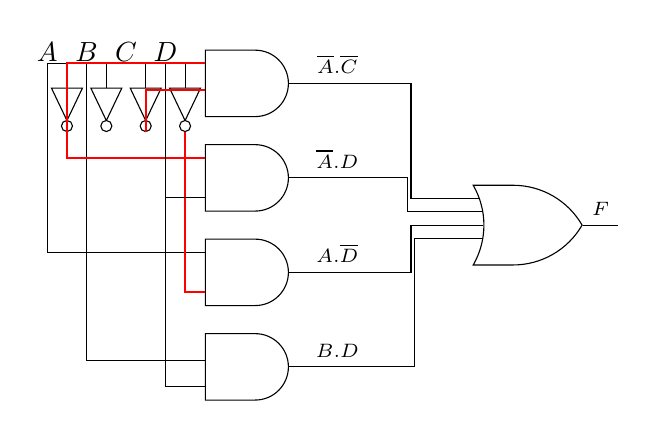
\begin{tikzpicture}

 %%Paramaters
%% var position, can be modified
\def\varPos{4.00}
\def\FunctionPos{6}
\node (x) at (0, \varPos) {$A$};
\node (y) at (0.5, \varPos) {$B$};
\node (z) at (1, \varPos) {$C$};
\node (w) at (1.5, \varPos) {$D$};

                \node[not gate US, draw, rotate=270] at ($(x) + (0.25, -0.6)$) (notx) {};
                \draw ($(x)+(0,-1ex)$) -| (notx.input); 
                \node[not gate US, draw, rotate=270] at ($(y) + (0.25, -0.6)$) (noty) {};
                \draw ($(y)+(0,-1ex)$) -| (noty.input); 
                \node[not gate US, draw, rotate=270] at ($(z) + (0.25, -0.6)$) (notz) {};
                \draw ($(z)+(0,-1ex)$) -| (notz.input);
                \node[not gate US, draw, rotate=270] at ($(w) + (0.25, -0.6)$) (notw) {};
                \draw ($(w)+(0,-1ex)$) -| (notw.input);
             

 %% ***Function  : Gate for term n° 1 [ B.D ]***
  
                \node[and gate US, draw, rotate=0, logic gate inputs=nnnn] at (2.5, 0.00) (xandy0) {};\draw (xandy0.output) -- node[above]{\scriptsize $ B.D $} ($(xandy0) + (1.8, 0)$);
                % Y
\draw ($(y) + (0, -1ex)$)|- (xandy0.input 2);
% W
\draw ($(w) + (0, -1ex)$)|- (xandy0.input 4);
 

 %% ***Function  : Gate for term n° 1 [ A.D' ]***
  
                \node[and gate US, draw, rotate=0, logic gate inputs=nnnn] at (2.5, 1.20) (xandy1) {};\draw (xandy1.output) -- node[above]{\scriptsize $ A.\overline{D} $} ($(xandy1) + (1.8, 0)$);
                % X
\draw ($(x) + (0, -1ex)$)|- (xandy1.input 1);
% W
\draw [line width=0.25mm,   red] (notw.output)
            -- ([xshift=0cm]notw.output) |- (xandy1.input 4);
 

 %% ***Function  : Gate for term n° 1 [ A'.D ]***
  
                \node[and gate US, draw, rotate=0, logic gate inputs=nnnn] at (2.5, 2.40) (xandy2) {};\draw (xandy2.output) -- node[above]{\scriptsize $ \overline{A}.D $} ($(xandy2) + (1.8, 0)$);
                % X
\draw [line width=0.25mm,   red] (notx.output)
            -- ([xshift=0cm]notx.output) |- (xandy2.input 1);
% W
\draw ($(w) + (0, -1ex)$)|- (xandy2.input 4);
 

 %% ***Function  : Gate for term n° 1 [ A'.C' ]***
  
                \node[and gate US, draw, rotate=0, logic gate inputs=nnnn] at (2.5, 3.60) (xandy3) {};\draw (xandy3.output) -- node[above]{\scriptsize $ \overline{A}.\overline{C} $} ($(xandy3) + (1.8, 0)$);
                % X
\draw [line width=0.25mm,   red] (notx.output)
            -- ([xshift=0cm]notx.output) |- (xandy3.input 1);
% Z
\draw [line width=0.25mm,   red] (notz.output)
            -- ([xshift=0cm]notz.output) |- (xandy3.input 3);


%% Function F Large OR Gate

\node[or gate US, draw, rotate=0, logic gate inputs=nnnnn] at (\FunctionPos, 1.80) (xory0) {};


            \draw (xory0.output) -- node[above]{\scriptsize $F$} ($(xory0.east) + (+3ex, 0)$);


            \draw (xandy0.output) -- ([xshift=1.60cm]xandy0.output) |- (xory0.input 4);

\draw (xandy1.output) -- ([xshift=1.55cm]xandy1.output) |- (xory0.input 3);

\draw (xandy2.output) -- ([xshift=1.50cm]xandy2.output) |- (xory0.input 2);

\draw (xandy3.output) -- ([xshift=1.55cm]xandy3.output) |- (xory0.input 1);

 \end{tikzpicture}




STRUCTURED LOGIGRAM-FILE-TEMPLATE






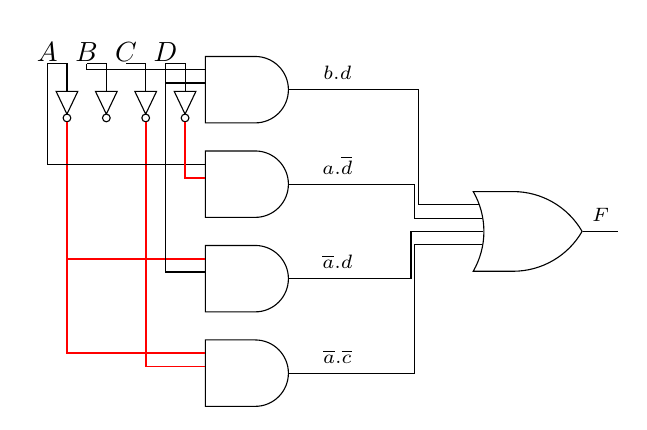
\begin{tikzpicture}

%%Paramaters
%% var position, can be modified
\def\varPos{ 4.08 }


\def\FunctionPos{6}



    \node (x1) at (0.0, \varPos) {$ A $};
    \node[not gate US, draw, rotate=270, scale=0.7] at ($(x1) + (0.25, -0.6)$) (notx1) {};
    
        \draw ($(x1)+(0,-1ex)$) -| (notx1.input);
    

    \node (x2) at (0.5, \varPos) {$ B $};
    \node[not gate US, draw, rotate=270, scale=0.7] at ($(x2) + (0.25, -0.6)$) (notx2) {};
    
        \draw ($(x2)+(0,-1ex)$) -| (notx2.input);
    

    \node (x3) at (1.0, \varPos) {$ C $};
    \node[not gate US, draw, rotate=270, scale=0.7] at ($(x3) + (0.25, -0.6)$) (notx3) {};
    
        \draw ($(x3)+(0,-1ex)$) -| (notx3.input);
    

    \node (x4) at (1.5, \varPos) {$ D $};
    \node[not gate US, draw, rotate=270, scale=0.7] at ($(x4) + (0.25, -0.6)$) (notx4) {};
    
        \draw ($(x4)+(0,-1ex)$) -| (notx4.input);
    








    
        
     %% ***Function F : Gate for term n° 1 [ {'default': "a'.c'", 'formatted': '\\overline{a}.\\overline{c}'} ]***
        
           \node[and gate US, draw, rotate=0, logic gate inputs=nnnn] at (2.5, 0.0) (xandyFg0) {};
           \draw (xandyFg0.output) -- node[above]{\scriptsize $ \overline{a}.\overline{c} $} ($(xandyFg0) + (1.8, 0)$);
        
        
            
                \draw [line width=0.25mm,   red] (notx1.output)
                -- ([xshift=0cm]notx1.output) |- (xandyFg0.input 1);
                
            
        
            
        
            
                \draw [line width=0.25mm,   red] (notx3.output)
                -- ([xshift=0cm]notx3.output) |- (xandyFg0.input 2);
                
            
        
            
        
        
     
    
        
     %% ***Function F : Gate for term n° 2 [ {'default': "a'.d", 'formatted': '\\overline{a}.d'} ]***
        
           \node[and gate US, draw, rotate=0, logic gate inputs=nnnn] at (2.5, 1.2) (xandyFg1) {};
           \draw (xandyFg1.output) -- node[above]{\scriptsize $ \overline{a}.d $} ($(xandyFg1) + (1.8, 0)$);
        
        
            
                \draw [line width=0.25mm,   red] (notx1.output)
                -- ([xshift=0cm]notx1.output) |- (xandyFg1.input 1);
                
            
        
            
        
            
        
            
                \draw ($(x4) + (0, -1ex)$)|- (xandyFg1.input 2);
                
            
        
        
     
    
        
     %% ***Function F : Gate for term n° 3 [ {'default': "a.d'", 'formatted': 'a.\\overline{d}'} ]***
        
           \node[and gate US, draw, rotate=0, logic gate inputs=nnnn] at (2.5, 2.4) (xandyFg2) {};
           \draw (xandyFg2.output) -- node[above]{\scriptsize $ a.\overline{d} $} ($(xandyFg2) + (1.8, 0)$);
        
        
            
                \draw ($(x1) + (0, -1ex)$)|- (xandyFg2.input 1);
                
            
        
            
        
            
        
            
                \draw [line width=0.25mm,   red] (notx4.output)
                -- ([xshift=0cm]notx4.output) |- (xandyFg2.input 2);
                
            
        
        
     
    
        
     %% ***Function F : Gate for term n° 4 [ {'default': 'b.d', 'formatted': 'b.d'} ]***
        
           \node[and gate US, draw, rotate=0, logic gate inputs=nnnn] at (2.5, 3.5999999999999996) (xandyFg3) {};
           \draw (xandyFg3.output) -- node[above]{\scriptsize $ b.d $} ($(xandyFg3) + (1.8, 0)$);
        
        
            
        
            
                \draw ($(x2) + (0, -1ex)$)|- (xandyFg3.input 1);
                
            
        
            
        
            
                \draw ($(x4) + (0, -1ex)$)|- (xandyFg3.input 2);
                
            
        
        
     
    


    %% y_pos : the position of OR gate according to their related gates
    

    %% Function F Large OR Gate
    

    
        \node[or gate US, draw, rotate=0, logic gate inputs=nnnnn] at (\FunctionPos, 1.7999999999999998) (xoryF) {};
        \draw (xoryF.output) -- node[above]{\scriptsize $F$} ($(xoryF.east) + (+3ex, 0)$);
    


    
    
    
    

        
            
             \draw (xandyFg0.output) -- ++(1.6,0) |- (xoryF.input 4);
            

        
        

    

        
            
             \draw (xandyFg1.output) -- ++(1.55,0) |- (xoryF.input 3);
            

        
        

    

        
            
             \draw (xandyFg2.output) -- ++(1.6,0) |- (xoryF.input 2);
            

        
        

    

        
            
             \draw (xandyFg3.output) -- ++(1.6500000000000001,0) |- (xoryF.input 1);
            

        
        

    


 \end{tikzpicture}




\pagebreak

\paragraph{Q1}

Convert the following numbers, \hfill\aRL{أنجز التحويلات الآتية}


$(915\,8988)_{ 2 } = (........)_{ 8}$



\hrule width 1\linewidth
\pagebreak

\subsection{Correction}


\paragraph{Q1}

Convert the following numbers, \hfill\aRL{أنجز التحويلات الآتية}


$(915\,8988)_{ 2 } = (  4274\,0514)_{ 8}$

\pagebreak

\paragraph{Q1}

Calculate  the following operations in base 8 :  أنجز العمليات الآتية في الأساس 8

\begin{verbatim}

  1012\,4064
- 245\,5447
-------------------

=  ........


\end{verbatim}


\hrule width 1\linewidth
\pagebreak

\subsection{Correction}


\paragraph{Q1}

Calculate  the following operations in base 8 :  أنجز العمليات الآتية في الأساس 8

\begin{verbatim}

  1012\,4064
- 245\,5447
-------------------

=  544\,6415


\end{verbatim}
\pagebreak

\paragraph{Q1}

Faire les conversion suivantes: NOT IMPLEMENTED (MESURE questions) 


\hrule width 1\linewidth
\pagebreak

\subsection{Correction}


\paragraph{Q1}

  10001111
+ 10011010
----------
 100101001

\pagebreak

\paragraph{Q1}



Etudier la fonction suivante:



Study the following function:

\begin{arab}[utf]
ادرس الدالة الآتية:
\end{arab}
$F(A,B,C,D) =$



 




\hrule width 1\linewidth
\pagebreak

\subsection{Correction}


\paragraph{Q1}



Etudier la fonction suivante:



Study the following function:

\begin{arab}[utf]
ادرس الدالة الآتية:
\end{arab}
$F(A,B,C,D) =$





$Fx0 = [15]$

\textbf{Don't Care }

$Fx0 = []$



\textbf{Truth Table \aRL{جدول الحقيقة}}



\begin{tabular}{|c|c|c|c||c|}
\hline
X & Y & Z & W & F \\

    
        \hline
    
  
  
  0 & 0 & 0 & 0 & 0 \\

    
  
  
  0 & 0 & 0 & 1 & 0 \\

    
  
  
  0 & 0 & 1 & 0 & 0 \\

    
  
  
  0 & 0 & 1 & 1 & 0 \\

    
        \hline
    
  
  
  0 & 1 & 0 & 0 & 0 \\

    
  
  
  0 & 1 & 0 & 1 & 0 \\

    
  
  
  0 & 1 & 1 & 0 & 0 \\

    
  
  
  0 & 1 & 1 & 1 & 0 \\

    
        \hline
    
  
  
  1 & 0 & 0 & 0 & 0 \\

    
  
  
  1 & 0 & 0 & 1 & 0 \\

    
  
  
  1 & 0 & 1 & 0 & 0 \\

    
  
  
  1 & 0 & 1 & 1 & 0 \\

    
        \hline
    
  
  
  1 & 1 & 0 & 0 & 0 \\

    
  
  
  1 & 1 & 0 & 1 & 0 \\

    
  
  
  1 & 1 & 1 & 0 & 0 \\

    
  
  
  1 & 1 & 1 & 1 & 1 \\

\hline
\end{tabular}


\textbf{Canonical Forms \aRL{الأشكال القانونية}}
\begin{itemize}
\item $Fx0(A,B,C,D) =  X.Y.Z.W$
\item $Fx0(A,B,C,D) = (X+Y+Z+W) . (X+Y+Z+\overline{W}) . (X+Y+\overline{Z}+W) . (X+Y+\overline{Z}+\overline{W}) . (X+\overline{Y}+Z+W) . (X+\overline{Y}+Z+\overline{W}) . (X+\overline{Y}+\overline{Z}+W) . (X+\overline{Y}+\overline{Z}+\overline{W}) . (\overline{X}+Y+Z+W) . (\overline{X}+Y+Z+\overline{W}) . (\overline{X}+Y+\overline{Z}+W) . (\overline{X}+Y+\overline{Z}+\overline{W}) . (\overline{X}+\overline{Y}+Z+W) . (\overline{X}+\overline{Y}+Z+\overline{W}) . (\overline{X}+\overline{Y}+\overline{Z}+W)$
 \item $Fx0(A,B,C,D) =  \sum(15)$
 \item $Fx0(A,B,C,D) =  \prod(0, 1, 2, 3, 4, 5, 6, 7, 8, 9, 10, 11, 12, 13, 14)$
\end{itemize}




 




\textbf{Karnaugh Table \aRL{جدول كارنوف}}

\begin{karnaugh-map}[4][4][1][ZW][XY]
  \minterms{ 15 }
  \maxterms{ 0, 1, 2, 3, 4, 5, 6, 7, 8, 9, 10, 11, 12, 13, 14 }
  

    \implicant{15}{15}

 \end{karnaugh-map}

    Simplified Sum of products : $ w.x.y.z $\\
    Simplified product of sums : $(w).(x).(y).(z)$

\textbf{Logic diagram \aRL{المخطط المنطقي}}

 \label{logigram-Fx0}
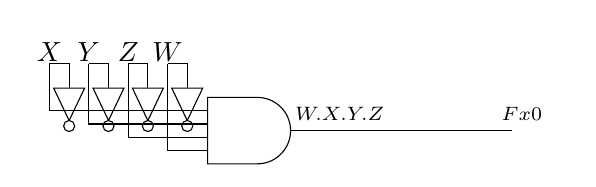
\begin{tikzpicture}

 %%Paramaters
%% var position, can be modified
\def\varPos{1.00}
\def\FunctionPos{6}
\node (x) at (0, \varPos) {$X$};
\node (y) at (0.5, \varPos) {$Y$};
\node (z) at (1, \varPos) {$Z$};
\node (w) at (1.5, \varPos) {$W$};

                \node[not gate US, draw, rotate=270] at ($(x) + (0.25, -0.6)$) (notx) {};
                \draw ($(x)+(0,-1ex)$) -| (notx.input); 
                \node[not gate US, draw, rotate=270] at ($(y) + (0.25, -0.6)$) (noty) {};
                \draw ($(y)+(0,-1ex)$) -| (noty.input); 
                \node[not gate US, draw, rotate=270] at ($(z) + (0.25, -0.6)$) (notz) {};
                \draw ($(z)+(0,-1ex)$) -| (notz.input);
                \node[not gate US, draw, rotate=270] at ($(w) + (0.25, -0.6)$) (notw) {};
                \draw ($(w)+(0,-1ex)$) -| (notw.input);
             

 %% ***Function  : Gate for term n° 1 [ W.X.Y.Z ]***
  
                \node[and gate US, draw, rotate=0, logic gate inputs=nnnn] at (2.5, 0.00) (xandy0) {};\draw (xandy0.output) -- node[above]{\scriptsize $ W.X.Y.Z $} ($(xandy0) + (1.8, 0)$);
                % X
\draw ($(x) + (0, -1ex)$)|- (xandy0.input 1);
% Y
\draw ($(y) + (0, -1ex)$)|- (xandy0.input 2);
% Z
\draw ($(z) + (0, -1ex)$)|- (xandy0.input 3);
% W
\draw ($(w) + (0, -1ex)$)|- (xandy0.input 4);


%% Function Fx0 Large OR Gate

\node at (\FunctionPos, 0.00) (xory0) {};


            \draw (xory0) node[above]{\scriptsize $Fx0$} ($(xory0.east) + (+3ex, 0)$);


            \draw (xandy0.output) -- ([xshift=1.60cm]xandy0.output) |- (xory0);

 \end{tikzpicture}




STRUCTURED LOGIGRAM-FILE-TEMPLATE






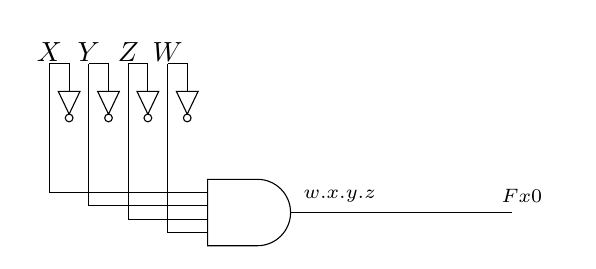
\begin{tikzpicture}

%%Paramaters
%% var position, can be modified
\def\varPos{ 2.04 }


\def\FunctionPos{6}



    \node (x1) at (0.0, \varPos) {$ X $};
    \node[not gate US, draw, rotate=270, scale=0.7] at ($(x1) + (0.25, -0.6)$) (notx1) {};
    
        \draw ($(x1)+(0,-1ex)$) -| (notx1.input);
    

    \node (x2) at (0.5, \varPos) {$ Y $};
    \node[not gate US, draw, rotate=270, scale=0.7] at ($(x2) + (0.25, -0.6)$) (notx2) {};
    
        \draw ($(x2)+(0,-1ex)$) -| (notx2.input);
    

    \node (x3) at (1.0, \varPos) {$ Z $};
    \node[not gate US, draw, rotate=270, scale=0.7] at ($(x3) + (0.25, -0.6)$) (notx3) {};
    
        \draw ($(x3)+(0,-1ex)$) -| (notx3.input);
    

    \node (x4) at (1.5, \varPos) {$ W $};
    \node[not gate US, draw, rotate=270, scale=0.7] at ($(x4) + (0.25, -0.6)$) (notx4) {};
    
        \draw ($(x4)+(0,-1ex)$) -| (notx4.input);
    








    
        
     %% ***Function Fx0 : Gate for term n° 1 [ {'default': 'w.x.y.z', 'formatted': 'w.x.y.z'} ]***
        
           \node[and gate US, draw, rotate=0, logic gate inputs=nnnn] at (2.5, 0.0) (xandyFx0g0) {};
           \draw (xandyFx0g0.output) -- node[above]{\scriptsize $ w.x.y.z $} ($(xandyFx0g0) + (1.8, 0)$);
        
        
            
                \draw ($(x1) + (0, -1ex)$)|- (xandyFx0g0.input 1);
                
            
        
            
                \draw ($(x2) + (0, -1ex)$)|- (xandyFx0g0.input 2);
                
            
        
            
                \draw ($(x3) + (0, -1ex)$)|- (xandyFx0g0.input 3);
                
            
        
            
                \draw ($(x4) + (0, -1ex)$)|- (xandyFx0g0.input 4);
                
            
        
        
     
    


    %% y_pos : the position of OR gate according to their related gates
    

    %% Function Fx0 Large OR Gate
    

    
        \node at (\FunctionPos, 0.0) (xoryFx0) {};
        \draw (xoryFx0)  node[above]{\scriptsize $Fx0$} ($(xoryFx0.east) + (+3ex, 0)$);
    


    
    
    
    

        
            
             \draw (xandyFx0g0.output) -- (xoryFx0);
            
        
        

    


 \end{tikzpicture}




\pagebreak

\paragraph{Q1}



Etudier le circuit suivant:



Study the following circuit:

\begin{arab}[utf]
ادرس الدارة الآتية:
\end{arab}

 

$Fx0 = [15]$



$F0 = [3, 5, 6, 7, 9, 10, 11, 12, 13, 14]$



$F1 = [1, 2, 4, 7, 8, 11, 13, 14]$



$F2 = [0, 1, 2, 3, 4, 5, 6, 7, 11, 12]$



$F3 = [0, 1, 2, 3, 4, 5, 6, 7]$



\textbf{Don't Care }
 
$Fx0 = []$

$F0 = []$

$F1 = []$

$F2 = []$

$F3 = []$



$F(A,B,C,D) =$



 






\hrule width 1\linewidth
\pagebreak

\subsection{Correction}


\paragraph{Q1}



Etudier le circuit suivant:



Study the following circuit:

\begin{arab}[utf]
ادرس الدارة الآتية:
\end{arab}

 

$Fx0 = [15]$



$F0 = [3, 5, 6, 7, 9, 10, 11, 12, 13, 14]$



$F1 = [1, 2, 4, 7, 8, 11, 13, 14]$



$F2 = [0, 1, 2, 3, 4, 5, 6, 7, 11, 12]$



$F3 = [0, 1, 2, 3, 4, 5, 6, 7]$



\textbf{Don't Care }
 
$Fx0 = []$

$F0 = []$

$F1 = []$

$F2 = []$

$F3 = []$



$F(A,B,C,D) =$







\textbf{Inputs and Outputs \aRL{المداخل والمخارج}}

\begin{itemize}
\item Inputs

    \begin{itemize}
    
        \item $X = 0 /1 $
    
        \item $Y = 0 /1 $
    
        \item $Z = 0 /1 $
    
        \item $W = 0 /1 $
    
    \end{itemize}
\item Outputs
    \begin{itemize}
    
        \item $Fx0 = 0 /1 $
    
        \item $F0 = 0 /1 $
    
        \item $F1 = 0 /1 $
    
        \item $F2 = 0 /1 $
    
        \item $F3 = 0 /1 $
    
    \end{itemize}
\end{itemize}

\textbf{Truth Table \aRL{جدول الحقيقة}}

\begin{tabular}{|c|c|c|c||c|c|c|c|c|}
\hline
X & Y & Z & W

  & Fx0

  & F0

  & F1

  & F2

  & F3
 \\
\hline

  
  
  0 & 0 & 0 & 0
  
    
    
    & 0
  
    
    
    & 0
  
    
    
    & 0
  
    
    
    & 1
  
    
    
    & 1
   \\
  

  
  
  0 & 0 & 0 & 1
  
    
    
    & 0
  
    
    
    & 0
  
    
    
    & 1
  
    
    
    & 1
  
    
    
    & 1
   \\
  

  
  
  0 & 0 & 1 & 0
  
    
    
    & 0
  
    
    
    & 0
  
    
    
    & 1
  
    
    
    & 1
  
    
    
    & 1
   \\
  

  
  
  0 & 0 & 1 & 1
  
    
    
    & 0
  
    
    
    & 1
  
    
    
    & 0
  
    
    
    & 1
  
    
    
    & 1
   \\
  \hline

  
  
  0 & 1 & 0 & 0
  
    
    
    & 0
  
    
    
    & 0
  
    
    
    & 1
  
    
    
    & 1
  
    
    
    & 1
   \\
  

  
  
  0 & 1 & 0 & 1
  
    
    
    & 0
  
    
    
    & 1
  
    
    
    & 0
  
    
    
    & 1
  
    
    
    & 1
   \\
  

  
  
  0 & 1 & 1 & 0
  
    
    
    & 0
  
    
    
    & 1
  
    
    
    & 0
  
    
    
    & 1
  
    
    
    & 1
   \\
  

  
  
  0 & 1 & 1 & 1
  
    
    
    & 0
  
    
    
    & 1
  
    
    
    & 1
  
    
    
    & 1
  
    
    
    & 1
   \\
  \hline

  
  
  1 & 0 & 0 & 0
  
    
    
    & 0
  
    
    
    & 0
  
    
    
    & 1
  
    
    
    & 0
  
    
    
    & 0
   \\
  

  
  
  1 & 0 & 0 & 1
  
    
    
    & 0
  
    
    
    & 1
  
    
    
    & 0
  
    
    
    & 0
  
    
    
    & 0
   \\
  

  
  
  1 & 0 & 1 & 0
  
    
    
    & 0
  
    
    
    & 1
  
    
    
    & 0
  
    
    
    & 0
  
    
    
    & 0
   \\
  

  
  
  1 & 0 & 1 & 1
  
    
    
    & 0
  
    
    
    & 1
  
    
    
    & 1
  
    
    
    & 1
  
    
    
    & 0
   \\
  \hline

  
  
  1 & 1 & 0 & 0
  
    
    
    & 0
  
    
    
    & 1
  
    
    
    & 0
  
    
    
    & 1
  
    
    
    & 0
   \\
  

  
  
  1 & 1 & 0 & 1
  
    
    
    & 0
  
    
    
    & 1
  
    
    
    & 1
  
    
    
    & 0
  
    
    
    & 0
   \\
  

  
  
  1 & 1 & 1 & 0
  
    
    
    & 0
  
    
    
    & 1
  
    
    
    & 1
  
    
    
    & 0
  
    
    
    & 0
   \\
  

  
  
  1 & 1 & 1 & 1
  
    
    
    & 1
  
    
    
    & 0
  
    
    
    & 0
  
    
    
    & 0
  
    
    
    & 0
   \\
  \hline

\end{tabular}



\textbf{Canonical Forms \aRL{الأشكال القانونية}}
\begin{itemize}
\item \textbf{First Canonical Forms \aRL{ الأشكال القانونية الأولى}}
    \begin{itemize}
    
        \item $Fx0(X, Y, Z, W) =  X.Y.Z.W$
    
        \item $F0(X, Y, Z, W) =  \overline{X}.\overline{Y}.Z.W + \overline{X}.Y.\overline{Z}.W + \overline{X}.Y.Z.\overline{W} + \overline{X}.Y.Z.W + X.\overline{Y}.\overline{Z}.W + X.\overline{Y}.Z.\overline{W} + X.\overline{Y}.Z.W + X.Y.\overline{Z}.\overline{W} + X.Y.\overline{Z}.W + X.Y.Z.\overline{W}$
    
        \item $F1(X, Y, Z, W) =  \overline{X}.\overline{Y}.\overline{Z}.W + \overline{X}.\overline{Y}.Z.\overline{W} + \overline{X}.Y.\overline{Z}.\overline{W} + \overline{X}.Y.Z.W + X.\overline{Y}.\overline{Z}.\overline{W} + X.\overline{Y}.Z.W + X.Y.\overline{Z}.W + X.Y.Z.\overline{W}$
    
        \item $F2(X, Y, Z, W) =  \overline{X}.\overline{Y}.\overline{Z}.\overline{W} + \overline{X}.\overline{Y}.\overline{Z}.W + \overline{X}.\overline{Y}.Z.\overline{W} + \overline{X}.\overline{Y}.Z.W + \overline{X}.Y.\overline{Z}.\overline{W} + \overline{X}.Y.\overline{Z}.W + \overline{X}.Y.Z.\overline{W} + \overline{X}.Y.Z.W + X.\overline{Y}.Z.W + X.Y.\overline{Z}.\overline{W}$
    
        \item $F3(X, Y, Z, W) =  \overline{X}.\overline{Y}.\overline{Z}.\overline{W} + \overline{X}.\overline{Y}.\overline{Z}.W + \overline{X}.\overline{Y}.Z.\overline{W} + \overline{X}.\overline{Y}.Z.W + \overline{X}.Y.\overline{Z}.\overline{W} + \overline{X}.Y.\overline{Z}.W + \overline{X}.Y.Z.\overline{W} + \overline{X}.Y.Z.W$
    
    \end{itemize}

\item \textbf{Second Canonical Forms \aRL{ الأشكال القانونية الثانية}}
    \begin{itemize}
    
        \item $Fx0(X, Y, Z, W) =  (X+Y+Z+W) . (X+Y+Z+\overline{W}) . (X+Y+\overline{Z}+W) . (X+Y+\overline{Z}+\overline{W}) . (X+\overline{Y}+Z+W) . (X+\overline{Y}+Z+\overline{W}) . (X+\overline{Y}+\overline{Z}+W) . (X+\overline{Y}+\overline{Z}+\overline{W}) . (\overline{X}+Y+Z+W) . (\overline{X}+Y+Z+\overline{W}) . (\overline{X}+Y+\overline{Z}+W) . (\overline{X}+Y+\overline{Z}+\overline{W}) . (\overline{X}+\overline{Y}+Z+W) . (\overline{X}+\overline{Y}+Z+\overline{W}) . (\overline{X}+\overline{Y}+\overline{Z}+W)$
    
        \item $F0(X, Y, Z, W) =  (X+Y+Z+W) . (X+Y+Z+\overline{W}) . (X+Y+\overline{Z}+W) . (X+\overline{Y}+Z+W) . (\overline{X}+Y+Z+W) . (\overline{X}+\overline{Y}+\overline{Z}+\overline{W})$
    
        \item $F1(X, Y, Z, W) =  (X+Y+Z+W) . (X+Y+\overline{Z}+\overline{W}) . (X+\overline{Y}+Z+\overline{W}) . (X+\overline{Y}+\overline{Z}+W) . (\overline{X}+Y+Z+\overline{W}) . (\overline{X}+Y+\overline{Z}+W) . (\overline{X}+\overline{Y}+Z+W) . (\overline{X}+\overline{Y}+\overline{Z}+\overline{W})$
    
        \item $F2(X, Y, Z, W) =  (\overline{X}+Y+Z+W) . (\overline{X}+Y+Z+\overline{W}) . (\overline{X}+Y+\overline{Z}+W) . (\overline{X}+\overline{Y}+Z+\overline{W}) . (\overline{X}+\overline{Y}+\overline{Z}+W) . (\overline{X}+\overline{Y}+\overline{Z}+\overline{W})$
    
        \item $F3(X, Y, Z, W) =  (\overline{X}+Y+Z+W) . (\overline{X}+Y+Z+\overline{W}) . (\overline{X}+Y+\overline{Z}+W) . (\overline{X}+Y+\overline{Z}+\overline{W}) . (\overline{X}+\overline{Y}+Z+W) . (\overline{X}+\overline{Y}+Z+\overline{W}) . (\overline{X}+\overline{Y}+\overline{Z}+W) . (\overline{X}+\overline{Y}+\overline{Z}+\overline{W})$
    
    \end{itemize}

\item \textbf{First Canonical Forms \aRL{ الأشكال القانونية الأولى}}
    \begin{itemize}
    
        \item $Fx0(X, Y, Z, W) = \sum(15)$
    
        \item $F0(X, Y, Z, W) = \sum(3, 5, 6, 7, 9, 10, 11, 12, 13, 14)$
    
        \item $F1(X, Y, Z, W) = \sum(1, 2, 4, 7, 8, 11, 13, 14)$
    
        \item $F2(X, Y, Z, W) = \sum(0, 1, 2, 3, 4, 5, 6, 7, 11, 12)$
    
        \item $F3(X, Y, Z, W) = \sum(0, 1, 2, 3, 4, 5, 6, 7)$
    
    \end{itemize}

\item \textbf{Second Canonical Forms \aRL{ الأشكال القانونية الثانية}}
    \begin{itemize}
    
        \item $Fx0(X, Y, Z, W) =  \prod(0, 1, 2, 3, 4, 5, 6, 7, 8, 9, 10, 11, 12, 13, 14)$
    
        \item $F0(X, Y, Z, W) =  \prod(0, 1, 2, 4, 8, 15)$
    
        \item $F1(X, Y, Z, W) =  \prod(0, 3, 5, 6, 9, 10, 12, 15)$
    
        \item $F2(X, Y, Z, W) =  \prod(8, 9, 10, 13, 14, 15)$
    
        \item $F3(X, Y, Z, W) =  \prod(8, 9, 10, 11, 12, 13, 14, 15)$
    
    \end{itemize}

\end{itemize}




 




\textbf{Karnaugh Table \aRL{جدول كارنوف}}

\begin{karnaugh-map}[4][4][1][ZW][XY]
  \minterms{ 15 }
  \maxterms{ 0, 1, 2, 3, 4, 5, 6, 7, 8, 9, 10, 11, 12, 13, 14 }
  
 
    \implicant{15}{15}
 
 \end{karnaugh-map}

    Simplified Sum of products : $Fx0 =  w.x.y.z $\\
    Simplified product of sums : $Fx0 = (w).(x).(y).(z)$


\begin{karnaugh-map}[4][4][1][ZW][XY]
  \minterms{ 3, 5, 6, 7, 9, 10, 11, 12, 13, 14 }
  \maxterms{ 0, 1, 2, 4, 8, 15 }
  
 
    \implicant{12}{13}
\implicant{10}{11}
\implicant{9}{11}
\implicant{6}{14}
\implicant{5}{13}
\implicant{3}{7}
 
 \end{karnaugh-map}

    Simplified Sum of products : $F0 =  w.x.\overline{y} + w.y.\overline{z} + w.\overline{x}.z + x.y.\overline{z} + x.\overline{y}.z + \overline{w}.y.z $\\
    Simplified product of sums : $F0 = (w+x+y).(w+x+z).(w+y+z).(x+y+z).(\overline{w}+\overline{x}+\overline{y}+\overline{z})$


\begin{karnaugh-map}[4][4][1][ZW][XY]
  \minterms{ 1, 2, 4, 7, 8, 11, 13, 14 }
  \maxterms{ 0, 3, 5, 6, 9, 10, 12, 15 }
  
 
    \implicant{14}{14}
\implicant{13}{13}
\implicant{11}{11}
\implicant{7}{7}
\implicant{8}{8}
\implicant{4}{4}
\implicant{2}{2}
\implicant{1}{1}
 
 \end{karnaugh-map}

    Simplified Sum of products : $F1 =  w.x.y.\overline{z} + w.x.\overline{y}.z + w.\overline{x}.y.z + \overline{w}.x.y.z + w.\overline{x}.\overline{y}.\overline{z} + \overline{w}.x.\overline{y}.\overline{z} + \overline{w}.\overline{x}.y.\overline{z} + \overline{w}.\overline{x}.\overline{y}.z $\\
    Simplified product of sums : $F1 = (w+x+y+z).(w+x+\overline{y}+\overline{z}).(w+\overline{x}+y+\overline{z}).(w+\overline{x}+\overline{y}+z).(\overline{w}+x+y+\overline{z}).(\overline{w}+x+\overline{y}+z).(\overline{w}+\overline{x}+y+z).(\overline{w}+\overline{x}+\overline{y}+\overline{z})$


\begin{karnaugh-map}[4][4][1][ZW][XY]
  \minterms{ 0, 1, 2, 3, 4, 5, 6, 7, 11, 12 }
  \maxterms{ 8, 9, 10, 13, 14, 15 }
  
 
    \implicant{0}{6}
\implicantedge{3}{3}{11}{11}
\implicant{4}{12}
 
 \end{karnaugh-map}

    Simplified Sum of products : $F2 =  \overline{x} + w.\overline{y}.z + \overline{w}.y.\overline{z} $\\
    Simplified product of sums : $F2 = (\overline{x}+y+z).(w+\overline{x}+\overline{z}).(\overline{w}+\overline{x}+\overline{y})$


\begin{karnaugh-map}[4][4][1][ZW][XY]
  \minterms{ 0, 1, 2, 3, 4, 5, 6, 7 }
  \maxterms{ 8, 9, 10, 11, 12, 13, 14, 15 }
  
 
    \implicant{0}{6}
 
 \end{karnaugh-map}

    Simplified Sum of products : $F3 =  \overline{x} $\\
    Simplified product of sums : $F3 = (\overline{x})$




\textbf{Ligc diagram \aRL{المخطط المنطقي}}

 \label{logigrammefonctionFx0-F0-F1-F2-F3}

 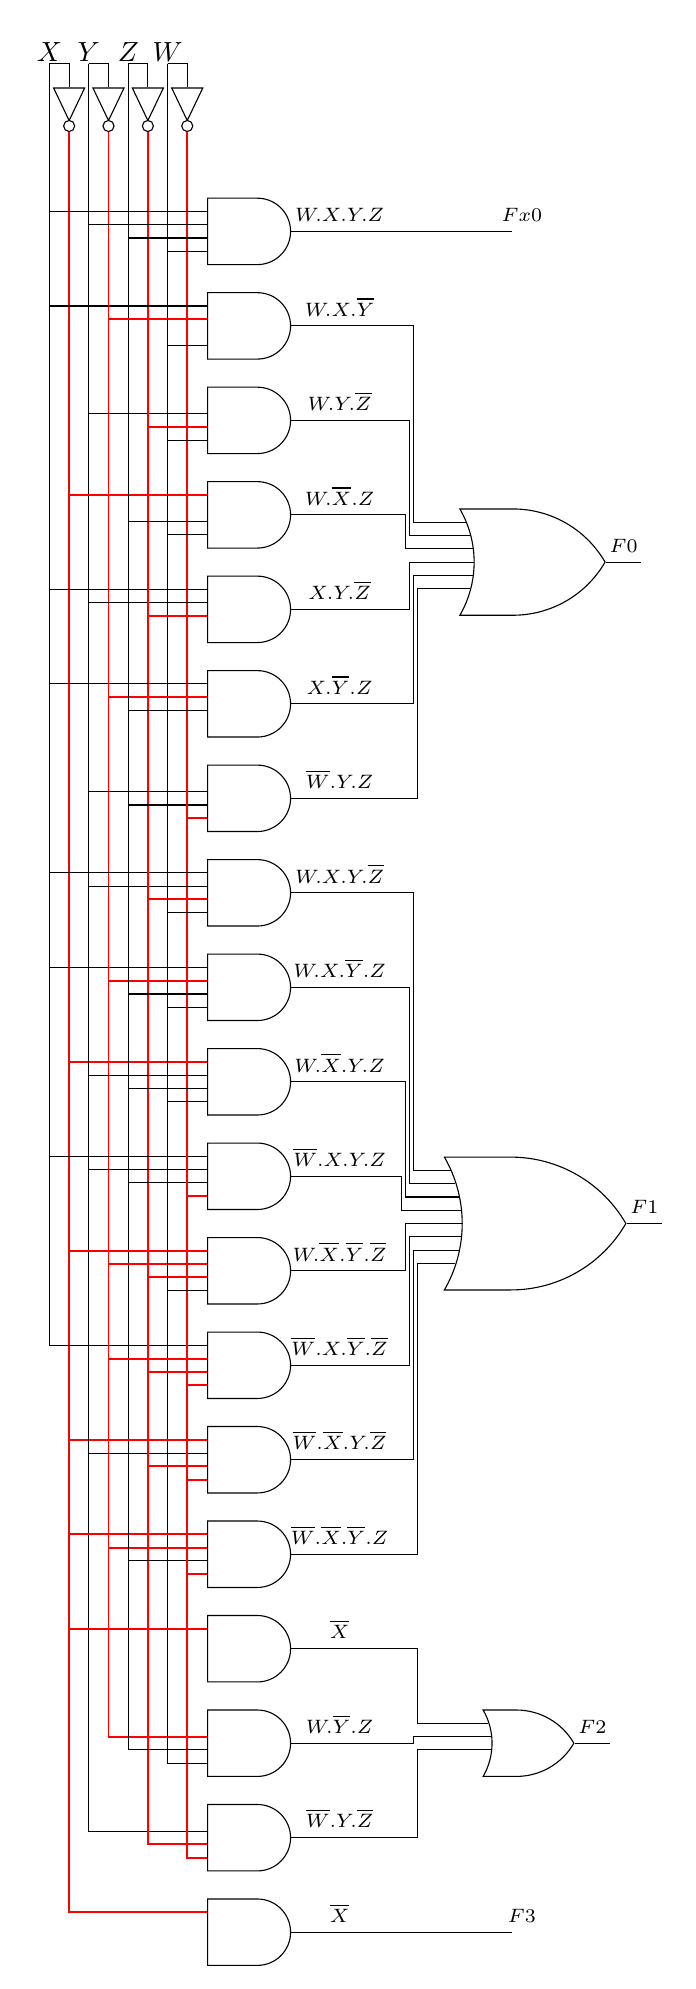
\begin{tikzpicture}

 %%Paramaters
%% var position, can be modified
\def\varPos{25.08}
\def\FunctionPos{6}
\node (x) at (0, \varPos) {$X$};
\node (y) at (0.5, \varPos) {$Y$};
\node (z) at (1, \varPos) {$Z$};
\node (w) at (1.5, \varPos) {$W$};

                \node[not gate US, draw, rotate=270] at ($(x) + (0.25, -0.6)$) (notx) {};
                \draw ($(x)+(0,-1ex)$) -| (notx.input); 
                \node[not gate US, draw, rotate=270] at ($(y) + (0.25, -0.6)$) (noty) {};
                \draw ($(y)+(0,-1ex)$) -| (noty.input); 
                \node[not gate US, draw, rotate=270] at ($(z) + (0.25, -0.6)$) (notz) {};
                \draw ($(z)+(0,-1ex)$) -| (notz.input);
                \node[not gate US, draw, rotate=270] at ($(w) + (0.25, -0.6)$) (notw) {};
                \draw ($(w)+(0,-1ex)$) -| (notw.input);
             

 %% ***Function F3 : Gate for term n° 1 [ X' ]***
  
                \node[and gate US, draw, rotate=0, logic gate inputs=nnnn] at (2.5, 1.20) (xandy1) {};\draw (xandy1.output) -- node[above]{\scriptsize $ \overline{X} $} ($(xandy1) + (1.8, 0)$);
                % X
\draw [line width=0.25mm,   red] (notx.output)
            -- ([xshift=0cm]notx.output) |- (xandy1.input 1);


%% Function F3 Large OR Gate

\node at (\FunctionPos, 1.20) (xory1) {};


            \draw (xory1) node[above]{\scriptsize $F3$} ($(xory1.east) + (+3ex, 0)$);


            \draw (xandy1.output) -- ([xshift=1.60cm]xandy1.output) |- (xory1);

 

 %% ***Function F2 : Gate for term n° 1 [ W'.Y.Z' ]***
  
                \node[and gate US, draw, rotate=0, logic gate inputs=nnnn] at (2.5, 2.40) (xandy2) {};\draw (xandy2.output) -- node[above]{\scriptsize $ \overline{W}.Y.\overline{Z} $} ($(xandy2) + (1.8, 0)$);
                % Y
\draw ($(y) + (0, -1ex)$)|- (xandy2.input 2);
% Z
\draw [line width=0.25mm,   red] (notz.output)
            -- ([xshift=0cm]notz.output) |- (xandy2.input 3);
% W
\draw [line width=0.25mm,   red] (notw.output)
            -- ([xshift=0cm]notw.output) |- (xandy2.input 4);
 

 %% ***Function F2 : Gate for term n° 2 [ W.Y'.Z ]***
  
                \node[and gate US, draw, rotate=0, logic gate inputs=nnnn] at (2.5, 3.60) (xandy3) {};\draw (xandy3.output) -- node[above]{\scriptsize $ W.\overline{Y}.Z $} ($(xandy3) + (1.8, 0)$);
                % Y
\draw [line width=0.25mm,   red] (noty.output)
            -- ([xshift=0cm]noty.output) |- (xandy3.input 2);
% Z
\draw ($(z) + (0, -1ex)$)|- (xandy3.input 3);
% W
\draw ($(w) + (0, -1ex)$)|- (xandy3.input 4);
 

 %% ***Function F2 : Gate for term n° 3 [ X' ]***
  
                \node[and gate US, draw, rotate=0, logic gate inputs=nnnn] at (2.5, 4.80) (xandy4) {};\draw (xandy4.output) -- node[above]{\scriptsize $ \overline{X} $} ($(xandy4) + (1.8, 0)$);
                % X
\draw [line width=0.25mm,   red] (notx.output)
            -- ([xshift=0cm]notx.output) |- (xandy4.input 1);


%% Function F2 Large OR Gate

\node[or gate US, draw, rotate=0, logic gate inputs=nnnn] at (\FunctionPos, 3.60) (xory2) {};


            \draw (xory2.output) -- node[above]{\scriptsize $F2$} ($(xory2.east) + (+3ex, 0)$);


            \draw (xandy2.output) -- ([xshift=1.60cm]xandy2.output) |- (xory2.input 3);

\draw (xandy3.output) -- ([xshift=1.55cm]xandy3.output) |- (xory2.input 2);

\draw (xandy4.output) -- ([xshift=1.60cm]xandy4.output) |- (xory2.input 1);

 

 %% ***Function F1 : Gate for term n° 1 [ W'.X'.Y'.Z ]***
  
                \node[and gate US, draw, rotate=0, logic gate inputs=nnnn] at (2.5, 6.00) (xandy5) {};\draw (xandy5.output) -- node[above]{\scriptsize $ \overline{W}.\overline{X}.\overline{Y}.Z $} ($(xandy5) + (1.8, 0)$);
                % X
\draw [line width=0.25mm,   red] (notx.output)
            -- ([xshift=0cm]notx.output) |- (xandy5.input 1);
% Y
\draw [line width=0.25mm,   red] (noty.output)
            -- ([xshift=0cm]noty.output) |- (xandy5.input 2);
% Z
\draw ($(z) + (0, -1ex)$)|- (xandy5.input 3);
% W
\draw [line width=0.25mm,   red] (notw.output)
            -- ([xshift=0cm]notw.output) |- (xandy5.input 4);
 

 %% ***Function F1 : Gate for term n° 2 [ W'.X'.Y.Z' ]***
  
                \node[and gate US, draw, rotate=0, logic gate inputs=nnnn] at (2.5, 7.20) (xandy6) {};\draw (xandy6.output) -- node[above]{\scriptsize $ \overline{W}.\overline{X}.Y.\overline{Z} $} ($(xandy6) + (1.8, 0)$);
                % X
\draw [line width=0.25mm,   red] (notx.output)
            -- ([xshift=0cm]notx.output) |- (xandy6.input 1);
% Y
\draw ($(y) + (0, -1ex)$)|- (xandy6.input 2);
% Z
\draw [line width=0.25mm,   red] (notz.output)
            -- ([xshift=0cm]notz.output) |- (xandy6.input 3);
% W
\draw [line width=0.25mm,   red] (notw.output)
            -- ([xshift=0cm]notw.output) |- (xandy6.input 4);
 

 %% ***Function F1 : Gate for term n° 3 [ W'.X.Y'.Z' ]***
  
                \node[and gate US, draw, rotate=0, logic gate inputs=nnnn] at (2.5, 8.40) (xandy7) {};\draw (xandy7.output) -- node[above]{\scriptsize $ \overline{W}.X.\overline{Y}.\overline{Z} $} ($(xandy7) + (1.8, 0)$);
                % X
\draw ($(x) + (0, -1ex)$)|- (xandy7.input 1);
% Y
\draw [line width=0.25mm,   red] (noty.output)
            -- ([xshift=0cm]noty.output) |- (xandy7.input 2);
% Z
\draw [line width=0.25mm,   red] (notz.output)
            -- ([xshift=0cm]notz.output) |- (xandy7.input 3);
% W
\draw [line width=0.25mm,   red] (notw.output)
            -- ([xshift=0cm]notw.output) |- (xandy7.input 4);
 

 %% ***Function F1 : Gate for term n° 4 [ W.X'.Y'.Z' ]***
  
                \node[and gate US, draw, rotate=0, logic gate inputs=nnnn] at (2.5, 9.60) (xandy8) {};\draw (xandy8.output) -- node[above]{\scriptsize $ W.\overline{X}.\overline{Y}.\overline{Z} $} ($(xandy8) + (1.8, 0)$);
                % X
\draw [line width=0.25mm,   red] (notx.output)
            -- ([xshift=0cm]notx.output) |- (xandy8.input 1);
% Y
\draw [line width=0.25mm,   red] (noty.output)
            -- ([xshift=0cm]noty.output) |- (xandy8.input 2);
% Z
\draw [line width=0.25mm,   red] (notz.output)
            -- ([xshift=0cm]notz.output) |- (xandy8.input 3);
% W
\draw ($(w) + (0, -1ex)$)|- (xandy8.input 4);
 

 %% ***Function F1 : Gate for term n° 5 [ W'.X.Y.Z ]***
  
                \node[and gate US, draw, rotate=0, logic gate inputs=nnnn] at (2.5, 10.80) (xandy9) {};\draw (xandy9.output) -- node[above]{\scriptsize $ \overline{W}.X.Y.Z $} ($(xandy9) + (1.8, 0)$);
                % X
\draw ($(x) + (0, -1ex)$)|- (xandy9.input 1);
% Y
\draw ($(y) + (0, -1ex)$)|- (xandy9.input 2);
% Z
\draw ($(z) + (0, -1ex)$)|- (xandy9.input 3);
% W
\draw [line width=0.25mm,   red] (notw.output)
            -- ([xshift=0cm]notw.output) |- (xandy9.input 4);
 

 %% ***Function F1 : Gate for term n° 6 [ W.X'.Y.Z ]***
  
                \node[and gate US, draw, rotate=0, logic gate inputs=nnnn] at (2.5, 12.00) (xandy10) {};\draw (xandy10.output) -- node[above]{\scriptsize $ W.\overline{X}.Y.Z $} ($(xandy10) + (1.8, 0)$);
                % X
\draw [line width=0.25mm,   red] (notx.output)
            -- ([xshift=0cm]notx.output) |- (xandy10.input 1);
% Y
\draw ($(y) + (0, -1ex)$)|- (xandy10.input 2);
% Z
\draw ($(z) + (0, -1ex)$)|- (xandy10.input 3);
% W
\draw ($(w) + (0, -1ex)$)|- (xandy10.input 4);
 

 %% ***Function F1 : Gate for term n° 7 [ W.X.Y'.Z ]***
  
                \node[and gate US, draw, rotate=0, logic gate inputs=nnnn] at (2.5, 13.20) (xandy11) {};\draw (xandy11.output) -- node[above]{\scriptsize $ W.X.\overline{Y}.Z $} ($(xandy11) + (1.8, 0)$);
                % X
\draw ($(x) + (0, -1ex)$)|- (xandy11.input 1);
% Y
\draw [line width=0.25mm,   red] (noty.output)
            -- ([xshift=0cm]noty.output) |- (xandy11.input 2);
% Z
\draw ($(z) + (0, -1ex)$)|- (xandy11.input 3);
% W
\draw ($(w) + (0, -1ex)$)|- (xandy11.input 4);
 

 %% ***Function F1 : Gate for term n° 8 [ W.X.Y.Z' ]***
  
                \node[and gate US, draw, rotate=0, logic gate inputs=nnnn] at (2.5, 14.40) (xandy12) {};\draw (xandy12.output) -- node[above]{\scriptsize $ W.X.Y.\overline{Z} $} ($(xandy12) + (1.8, 0)$);
                % X
\draw ($(x) + (0, -1ex)$)|- (xandy12.input 1);
% Y
\draw ($(y) + (0, -1ex)$)|- (xandy12.input 2);
% Z
\draw [line width=0.25mm,   red] (notz.output)
            -- ([xshift=0cm]notz.output) |- (xandy12.input 3);
% W
\draw ($(w) + (0, -1ex)$)|- (xandy12.input 4);


%% Function F1 Large OR Gate

\node[or gate US, draw, rotate=0, logic gate inputs=nnnnnnnnn] at (\FunctionPos, 10.20) (xory5) {};


            \draw (xory5.output) -- node[above]{\scriptsize $F1$} ($(xory5.east) + (+3ex, 0)$);


            \draw (xandy5.output) -- ([xshift=1.60cm]xandy5.output) |- (xory5.input 8);

\draw (xandy6.output) -- ([xshift=1.55cm]xandy6.output) |- (xory5.input 7);

\draw (xandy7.output) -- ([xshift=1.50cm]xandy7.output) |- (xory5.input 6);

\draw (xandy8.output) -- ([xshift=1.45cm]xandy8.output) |- (xory5.input 5);

\draw (xandy9.output) -- ([xshift=1.40cm]xandy9.output) |- (xory5.input 4);

\draw (xandy10.output) -- ([xshift=1.45cm]xandy10.output) |- (xory5.input 3);

\draw (xandy11.output) -- ([xshift=1.50cm]xandy11.output) |- (xory5.input 2);

\draw (xandy12.output) -- ([xshift=1.55cm]xandy12.output) |- (xory5.input 1);

 

 %% ***Function F0 : Gate for term n° 1 [ W'.Y.Z ]***
  
                \node[and gate US, draw, rotate=0, logic gate inputs=nnnn] at (2.5, 15.60) (xandy13) {};\draw (xandy13.output) -- node[above]{\scriptsize $ \overline{W}.Y.Z $} ($(xandy13) + (1.8, 0)$);
                % Y
\draw ($(y) + (0, -1ex)$)|- (xandy13.input 2);
% Z
\draw ($(z) + (0, -1ex)$)|- (xandy13.input 3);
% W
\draw [line width=0.25mm,   red] (notw.output)
            -- ([xshift=0cm]notw.output) |- (xandy13.input 4);
 

 %% ***Function F0 : Gate for term n° 2 [ X.Y'.Z ]***
  
                \node[and gate US, draw, rotate=0, logic gate inputs=nnnn] at (2.5, 16.80) (xandy14) {};\draw (xandy14.output) -- node[above]{\scriptsize $ X.\overline{Y}.Z $} ($(xandy14) + (1.8, 0)$);
                % X
\draw ($(x) + (0, -1ex)$)|- (xandy14.input 1);
% Y
\draw [line width=0.25mm,   red] (noty.output)
            -- ([xshift=0cm]noty.output) |- (xandy14.input 2);
% Z
\draw ($(z) + (0, -1ex)$)|- (xandy14.input 3);
 

 %% ***Function F0 : Gate for term n° 3 [ X.Y.Z' ]***
  
                \node[and gate US, draw, rotate=0, logic gate inputs=nnnn] at (2.5, 18.00) (xandy15) {};\draw (xandy15.output) -- node[above]{\scriptsize $ X.Y.\overline{Z} $} ($(xandy15) + (1.8, 0)$);
                % X
\draw ($(x) + (0, -1ex)$)|- (xandy15.input 1);
% Y
\draw ($(y) + (0, -1ex)$)|- (xandy15.input 2);
% Z
\draw [line width=0.25mm,   red] (notz.output)
            -- ([xshift=0cm]notz.output) |- (xandy15.input 3);
 

 %% ***Function F0 : Gate for term n° 4 [ W.X'.Z ]***
  
                \node[and gate US, draw, rotate=0, logic gate inputs=nnnn] at (2.5, 19.20) (xandy16) {};\draw (xandy16.output) -- node[above]{\scriptsize $ W.\overline{X}.Z $} ($(xandy16) + (1.8, 0)$);
                % X
\draw [line width=0.25mm,   red] (notx.output)
            -- ([xshift=0cm]notx.output) |- (xandy16.input 1);
% Z
\draw ($(z) + (0, -1ex)$)|- (xandy16.input 3);
% W
\draw ($(w) + (0, -1ex)$)|- (xandy16.input 4);
 

 %% ***Function F0 : Gate for term n° 5 [ W.Y.Z' ]***
  
                \node[and gate US, draw, rotate=0, logic gate inputs=nnnn] at (2.5, 20.40) (xandy17) {};\draw (xandy17.output) -- node[above]{\scriptsize $ W.Y.\overline{Z} $} ($(xandy17) + (1.8, 0)$);
                % Y
\draw ($(y) + (0, -1ex)$)|- (xandy17.input 2);
% Z
\draw [line width=0.25mm,   red] (notz.output)
            -- ([xshift=0cm]notz.output) |- (xandy17.input 3);
% W
\draw ($(w) + (0, -1ex)$)|- (xandy17.input 4);
 

 %% ***Function F0 : Gate for term n° 6 [ W.X.Y' ]***
  
                \node[and gate US, draw, rotate=0, logic gate inputs=nnnn] at (2.5, 21.60) (xandy18) {};\draw (xandy18.output) -- node[above]{\scriptsize $ W.X.\overline{Y} $} ($(xandy18) + (1.8, 0)$);
                % X
\draw ($(x) + (0, -1ex)$)|- (xandy18.input 1);
% Y
\draw [line width=0.25mm,   red] (noty.output)
            -- ([xshift=0cm]noty.output) |- (xandy18.input 2);
% W
\draw ($(w) + (0, -1ex)$)|- (xandy18.input 4);


%% Function F0 Large OR Gate

\node[or gate US, draw, rotate=0, logic gate inputs=nnnnnnn] at (\FunctionPos, 18.60) (xory13) {};


            \draw (xory13.output) -- node[above]{\scriptsize $F0$} ($(xory13.east) + (+3ex, 0)$);


            \draw (xandy13.output) -- ([xshift=1.60cm]xandy13.output) |- (xory13.input 6);

\draw (xandy14.output) -- ([xshift=1.55cm]xandy14.output) |- (xory13.input 5);

\draw (xandy15.output) -- ([xshift=1.50cm]xandy15.output) |- (xory13.input 4);

\draw (xandy16.output) -- ([xshift=1.45cm]xandy16.output) |- (xory13.input 3);

\draw (xandy17.output) -- ([xshift=1.50cm]xandy17.output) |- (xory13.input 2);

\draw (xandy18.output) -- ([xshift=1.55cm]xandy18.output) |- (xory13.input 1);

 

 %% ***Function Fx0 : Gate for term n° 1 [ W.X.Y.Z ]***
  
                \node[and gate US, draw, rotate=0, logic gate inputs=nnnn] at (2.5, 22.80) (xandy19) {};\draw (xandy19.output) -- node[above]{\scriptsize $ W.X.Y.Z $} ($(xandy19) + (1.8, 0)$);
                % X
\draw ($(x) + (0, -1ex)$)|- (xandy19.input 1);
% Y
\draw ($(y) + (0, -1ex)$)|- (xandy19.input 2);
% Z
\draw ($(z) + (0, -1ex)$)|- (xandy19.input 3);
% W
\draw ($(w) + (0, -1ex)$)|- (xandy19.input 4);


%% Function Fx0 Large OR Gate

\node at (\FunctionPos, 22.80) (xory19) {};


            \draw (xory19) node[above]{\scriptsize $Fx0$} ($(xory19.east) + (+3ex, 0)$);


            \draw (xandy19.output) -- ([xshift=1.60cm]xandy19.output) |- (xory19);

 \end{tikzpicture}





STRUCTURED LOGIGRAM-FILE-TEMPLATE






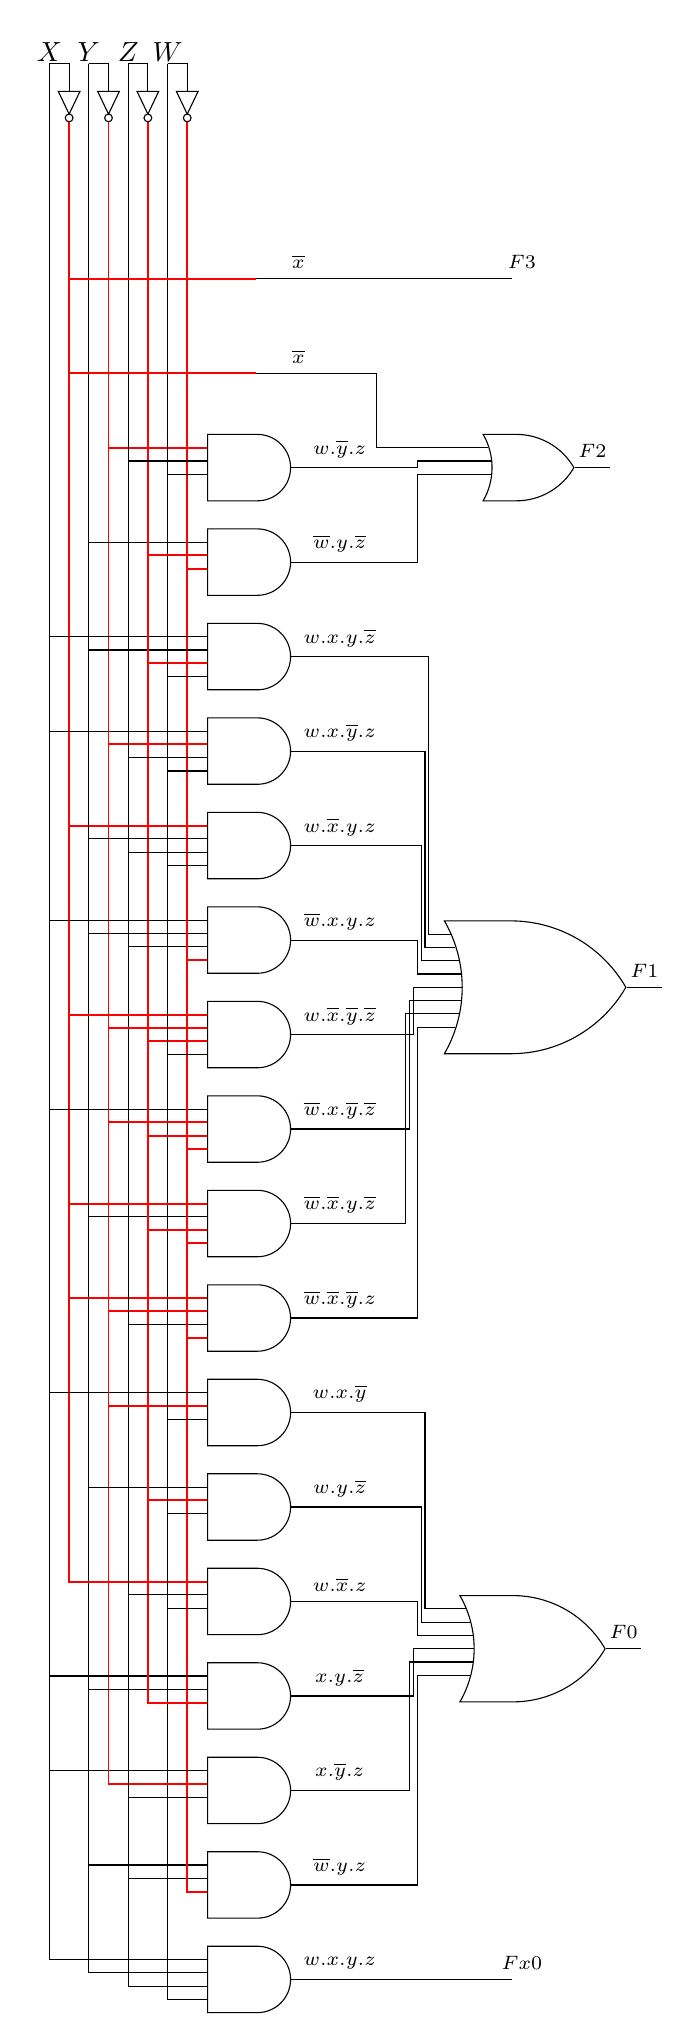
\begin{tikzpicture}

%%Paramaters
%% var position, can be modified
\def\varPos{ 24.48 }


\def\FunctionPos{6}



    \node (x1) at (0.0, \varPos) {$ X $};
    \node[not gate US, draw, rotate=270, scale=0.7] at ($(x1) + (0.25, -0.6)$) (notx1) {};
    
        \draw ($(x1)+(0,-1ex)$) -| (notx1.input);
    

    \node (x2) at (0.5, \varPos) {$ Y $};
    \node[not gate US, draw, rotate=270, scale=0.7] at ($(x2) + (0.25, -0.6)$) (notx2) {};
    
        \draw ($(x2)+(0,-1ex)$) -| (notx2.input);
    

    \node (x3) at (1.0, \varPos) {$ Z $};
    \node[not gate US, draw, rotate=270, scale=0.7] at ($(x3) + (0.25, -0.6)$) (notx3) {};
    
        \draw ($(x3)+(0,-1ex)$) -| (notx3.input);
    

    \node (x4) at (1.5, \varPos) {$ W $};
    \node[not gate US, draw, rotate=270, scale=0.7] at ($(x4) + (0.25, -0.6)$) (notx4) {};
    
        \draw ($(x4)+(0,-1ex)$) -| (notx4.input);
    








    
        
     %% ***Function Fx0 : Gate for term n° 1 [ {'default': 'w.x.y.z', 'formatted': 'w.x.y.z'} ]***
        
           \node[and gate US, draw, rotate=0, logic gate inputs=nnnn] at (2.5, 0.0) (xandyFx0g0) {};
           \draw (xandyFx0g0.output) -- node[above]{\scriptsize $ w.x.y.z $} ($(xandyFx0g0) + (1.8, 0)$);
        
        
            
                \draw ($(x1) + (0, -1ex)$)|- (xandyFx0g0.input 1);
                
            
        
            
                \draw ($(x2) + (0, -1ex)$)|- (xandyFx0g0.input 2);
                
            
        
            
                \draw ($(x3) + (0, -1ex)$)|- (xandyFx0g0.input 3);
                
            
        
            
                \draw ($(x4) + (0, -1ex)$)|- (xandyFx0g0.input 4);
                
            
        
        
     
    


    %% y_pos : the position of OR gate according to their related gates
    

    %% Function Fx0 Large OR Gate
    

    
        \node at (\FunctionPos, 0.0) (xoryFx0) {};
        \draw (xoryFx0)  node[above]{\scriptsize $Fx0$} ($(xoryFx0.east) + (+3ex, 0)$);
    


    
    
    
    

        
            
             \draw (xandyFx0g0.output) -- (xoryFx0);
            
        
        

    

    
        
     %% ***Function F0 : Gate for term n° 1 [ {'default': "w'.y.z", 'formatted': '\\overline{w}.y.z'} ]***
        
           \node[and gate US, draw, rotate=0, logic gate inputs=nnnn] at (2.5, 1.2) (xandyF0g0) {};
           \draw (xandyF0g0.output) -- node[above]{\scriptsize $ \overline{w}.y.z $} ($(xandyF0g0) + (1.8, 0)$);
        
        
            
        
            
                \draw ($(x2) + (0, -1ex)$)|- (xandyF0g0.input 1);
                
            
        
            
                \draw ($(x3) + (0, -1ex)$)|- (xandyF0g0.input 2);
                
            
        
            
                \draw [line width=0.25mm,   red] (notx4.output)
                -- ([xshift=0cm]notx4.output) |- (xandyF0g0.input 3);
                
            
        
        
     
    
        
     %% ***Function F0 : Gate for term n° 2 [ {'default': "x.y'.z", 'formatted': 'x.\\overline{y}.z'} ]***
        
           \node[and gate US, draw, rotate=0, logic gate inputs=nnnn] at (2.5, 2.4) (xandyF0g1) {};
           \draw (xandyF0g1.output) -- node[above]{\scriptsize $ x.\overline{y}.z $} ($(xandyF0g1) + (1.8, 0)$);
        
        
            
                \draw ($(x1) + (0, -1ex)$)|- (xandyF0g1.input 1);
                
            
        
            
                \draw [line width=0.25mm,   red] (notx2.output)
                -- ([xshift=0cm]notx2.output) |- (xandyF0g1.input 2);
                
            
        
            
                \draw ($(x3) + (0, -1ex)$)|- (xandyF0g1.input 3);
                
            
        
            
        
        
     
    
        
     %% ***Function F0 : Gate for term n° 3 [ {'default': "x.y.z'", 'formatted': 'x.y.\\overline{z}'} ]***
        
           \node[and gate US, draw, rotate=0, logic gate inputs=nnnn] at (2.5, 3.5999999999999996) (xandyF0g2) {};
           \draw (xandyF0g2.output) -- node[above]{\scriptsize $ x.y.\overline{z} $} ($(xandyF0g2) + (1.8, 0)$);
        
        
            
                \draw ($(x1) + (0, -1ex)$)|- (xandyF0g2.input 1);
                
            
        
            
                \draw ($(x2) + (0, -1ex)$)|- (xandyF0g2.input 2);
                
            
        
            
                \draw [line width=0.25mm,   red] (notx3.output)
                -- ([xshift=0cm]notx3.output) |- (xandyF0g2.input 3);
                
            
        
            
        
        
     
    
        
     %% ***Function F0 : Gate for term n° 4 [ {'default': "w.x'.z", 'formatted': 'w.\\overline{x}.z'} ]***
        
           \node[and gate US, draw, rotate=0, logic gate inputs=nnnn] at (2.5, 4.8) (xandyF0g3) {};
           \draw (xandyF0g3.output) -- node[above]{\scriptsize $ w.\overline{x}.z $} ($(xandyF0g3) + (1.8, 0)$);
        
        
            
                \draw [line width=0.25mm,   red] (notx1.output)
                -- ([xshift=0cm]notx1.output) |- (xandyF0g3.input 1);
                
            
        
            
        
            
                \draw ($(x3) + (0, -1ex)$)|- (xandyF0g3.input 2);
                
            
        
            
                \draw ($(x4) + (0, -1ex)$)|- (xandyF0g3.input 3);
                
            
        
        
     
    
        
     %% ***Function F0 : Gate for term n° 5 [ {'default': "w.y.z'", 'formatted': 'w.y.\\overline{z}'} ]***
        
           \node[and gate US, draw, rotate=0, logic gate inputs=nnnn] at (2.5, 6.0) (xandyF0g4) {};
           \draw (xandyF0g4.output) -- node[above]{\scriptsize $ w.y.\overline{z} $} ($(xandyF0g4) + (1.8, 0)$);
        
        
            
        
            
                \draw ($(x2) + (0, -1ex)$)|- (xandyF0g4.input 1);
                
            
        
            
                \draw [line width=0.25mm,   red] (notx3.output)
                -- ([xshift=0cm]notx3.output) |- (xandyF0g4.input 2);
                
            
        
            
                \draw ($(x4) + (0, -1ex)$)|- (xandyF0g4.input 3);
                
            
        
        
     
    
        
     %% ***Function F0 : Gate for term n° 6 [ {'default': "w.x.y'", 'formatted': 'w.x.\\overline{y}'} ]***
        
           \node[and gate US, draw, rotate=0, logic gate inputs=nnnn] at (2.5, 7.199999999999999) (xandyF0g5) {};
           \draw (xandyF0g5.output) -- node[above]{\scriptsize $ w.x.\overline{y} $} ($(xandyF0g5) + (1.8, 0)$);
        
        
            
                \draw ($(x1) + (0, -1ex)$)|- (xandyF0g5.input 1);
                
            
        
            
                \draw [line width=0.25mm,   red] (notx2.output)
                -- ([xshift=0cm]notx2.output) |- (xandyF0g5.input 2);
                
            
        
            
        
            
                \draw ($(x4) + (0, -1ex)$)|- (xandyF0g5.input 3);
                
            
        
        
     
    


    %% y_pos : the position of OR gate according to their related gates
    

    %% Function F0 Large OR Gate
    

    
        \node[or gate US, draw, rotate=0, logic gate inputs=nnnnnnn] at (\FunctionPos, 4.2) (xoryF0) {};
        \draw (xoryF0.output) -- node[above]{\scriptsize $F0$} ($(xoryF0.east) + (+3ex, 0)$);
    


    
    
    
    

        
            
             \draw (xandyF0g0.output) -- ++(1.6,0) |- (xoryF0.input 6);
            

        
        

    

        
            
             \draw (xandyF0g1.output) -- ++(1.5,0) |- (xoryF0.input 5);
            

        
        

    

        
            
             \draw (xandyF0g2.output) -- ++(1.55,0) |- (xoryF0.input 4);
            

        
        

    

        
            
             \draw (xandyF0g3.output) -- ++(1.6,0) |- (xoryF0.input 3);
            

        
        

    

        
            
             \draw (xandyF0g4.output) -- ++(1.6500000000000001,0) |- (xoryF0.input 2);
            

        
        

    

        
            
             \draw (xandyF0g5.output) -- ++(1.7000000000000002,0) |- (xoryF0.input 1);
            

        
        

    

    
        
     %% ***Function F1 : Gate for term n° 1 [ {'default': "w'.x'.y'.z", 'formatted': '\\overline{w}.\\overline{x}.\\overline{y}.z'} ]***
        
           \node[and gate US, draw, rotate=0, logic gate inputs=nnnn] at (2.5, 8.4) (xandyF1g0) {};
           \draw (xandyF1g0.output) -- node[above]{\scriptsize $ \overline{w}.\overline{x}.\overline{y}.z $} ($(xandyF1g0) + (1.8, 0)$);
        
        
            
                \draw [line width=0.25mm,   red] (notx1.output)
                -- ([xshift=0cm]notx1.output) |- (xandyF1g0.input 1);
                
            
        
            
                \draw [line width=0.25mm,   red] (notx2.output)
                -- ([xshift=0cm]notx2.output) |- (xandyF1g0.input 2);
                
            
        
            
                \draw ($(x3) + (0, -1ex)$)|- (xandyF1g0.input 3);
                
            
        
            
                \draw [line width=0.25mm,   red] (notx4.output)
                -- ([xshift=0cm]notx4.output) |- (xandyF1g0.input 4);
                
            
        
        
     
    
        
     %% ***Function F1 : Gate for term n° 2 [ {'default': "w'.x'.y.z'", 'formatted': '\\overline{w}.\\overline{x}.y.\\overline{z}'} ]***
        
           \node[and gate US, draw, rotate=0, logic gate inputs=nnnn] at (2.5, 9.6) (xandyF1g1) {};
           \draw (xandyF1g1.output) -- node[above]{\scriptsize $ \overline{w}.\overline{x}.y.\overline{z} $} ($(xandyF1g1) + (1.8, 0)$);
        
        
            
                \draw [line width=0.25mm,   red] (notx1.output)
                -- ([xshift=0cm]notx1.output) |- (xandyF1g1.input 1);
                
            
        
            
                \draw ($(x2) + (0, -1ex)$)|- (xandyF1g1.input 2);
                
            
        
            
                \draw [line width=0.25mm,   red] (notx3.output)
                -- ([xshift=0cm]notx3.output) |- (xandyF1g1.input 3);
                
            
        
            
                \draw [line width=0.25mm,   red] (notx4.output)
                -- ([xshift=0cm]notx4.output) |- (xandyF1g1.input 4);
                
            
        
        
     
    
        
     %% ***Function F1 : Gate for term n° 3 [ {'default': "w'.x.y'.z'", 'formatted': '\\overline{w}.x.\\overline{y}.\\overline{z}'} ]***
        
           \node[and gate US, draw, rotate=0, logic gate inputs=nnnn] at (2.5, 10.799999999999999) (xandyF1g2) {};
           \draw (xandyF1g2.output) -- node[above]{\scriptsize $ \overline{w}.x.\overline{y}.\overline{z} $} ($(xandyF1g2) + (1.8, 0)$);
        
        
            
                \draw ($(x1) + (0, -1ex)$)|- (xandyF1g2.input 1);
                
            
        
            
                \draw [line width=0.25mm,   red] (notx2.output)
                -- ([xshift=0cm]notx2.output) |- (xandyF1g2.input 2);
                
            
        
            
                \draw [line width=0.25mm,   red] (notx3.output)
                -- ([xshift=0cm]notx3.output) |- (xandyF1g2.input 3);
                
            
        
            
                \draw [line width=0.25mm,   red] (notx4.output)
                -- ([xshift=0cm]notx4.output) |- (xandyF1g2.input 4);
                
            
        
        
     
    
        
     %% ***Function F1 : Gate for term n° 4 [ {'default': "w.x'.y'.z'", 'formatted': 'w.\\overline{x}.\\overline{y}.\\overline{z}'} ]***
        
           \node[and gate US, draw, rotate=0, logic gate inputs=nnnn] at (2.5, 12.0) (xandyF1g3) {};
           \draw (xandyF1g3.output) -- node[above]{\scriptsize $ w.\overline{x}.\overline{y}.\overline{z} $} ($(xandyF1g3) + (1.8, 0)$);
        
        
            
                \draw [line width=0.25mm,   red] (notx1.output)
                -- ([xshift=0cm]notx1.output) |- (xandyF1g3.input 1);
                
            
        
            
                \draw [line width=0.25mm,   red] (notx2.output)
                -- ([xshift=0cm]notx2.output) |- (xandyF1g3.input 2);
                
            
        
            
                \draw [line width=0.25mm,   red] (notx3.output)
                -- ([xshift=0cm]notx3.output) |- (xandyF1g3.input 3);
                
            
        
            
                \draw ($(x4) + (0, -1ex)$)|- (xandyF1g3.input 4);
                
            
        
        
     
    
        
     %% ***Function F1 : Gate for term n° 5 [ {'default': "w'.x.y.z", 'formatted': '\\overline{w}.x.y.z'} ]***
        
           \node[and gate US, draw, rotate=0, logic gate inputs=nnnn] at (2.5, 13.2) (xandyF1g4) {};
           \draw (xandyF1g4.output) -- node[above]{\scriptsize $ \overline{w}.x.y.z $} ($(xandyF1g4) + (1.8, 0)$);
        
        
            
                \draw ($(x1) + (0, -1ex)$)|- (xandyF1g4.input 1);
                
            
        
            
                \draw ($(x2) + (0, -1ex)$)|- (xandyF1g4.input 2);
                
            
        
            
                \draw ($(x3) + (0, -1ex)$)|- (xandyF1g4.input 3);
                
            
        
            
                \draw [line width=0.25mm,   red] (notx4.output)
                -- ([xshift=0cm]notx4.output) |- (xandyF1g4.input 4);
                
            
        
        
     
    
        
     %% ***Function F1 : Gate for term n° 6 [ {'default': "w.x'.y.z", 'formatted': 'w.\\overline{x}.y.z'} ]***
        
           \node[and gate US, draw, rotate=0, logic gate inputs=nnnn] at (2.5, 14.399999999999999) (xandyF1g5) {};
           \draw (xandyF1g5.output) -- node[above]{\scriptsize $ w.\overline{x}.y.z $} ($(xandyF1g5) + (1.8, 0)$);
        
        
            
                \draw [line width=0.25mm,   red] (notx1.output)
                -- ([xshift=0cm]notx1.output) |- (xandyF1g5.input 1);
                
            
        
            
                \draw ($(x2) + (0, -1ex)$)|- (xandyF1g5.input 2);
                
            
        
            
                \draw ($(x3) + (0, -1ex)$)|- (xandyF1g5.input 3);
                
            
        
            
                \draw ($(x4) + (0, -1ex)$)|- (xandyF1g5.input 4);
                
            
        
        
     
    
        
     %% ***Function F1 : Gate for term n° 7 [ {'default': "w.x.y'.z", 'formatted': 'w.x.\\overline{y}.z'} ]***
        
           \node[and gate US, draw, rotate=0, logic gate inputs=nnnn] at (2.5, 15.6) (xandyF1g6) {};
           \draw (xandyF1g6.output) -- node[above]{\scriptsize $ w.x.\overline{y}.z $} ($(xandyF1g6) + (1.8, 0)$);
        
        
            
                \draw ($(x1) + (0, -1ex)$)|- (xandyF1g6.input 1);
                
            
        
            
                \draw [line width=0.25mm,   red] (notx2.output)
                -- ([xshift=0cm]notx2.output) |- (xandyF1g6.input 2);
                
            
        
            
                \draw ($(x3) + (0, -1ex)$)|- (xandyF1g6.input 3);
                
            
        
            
                \draw ($(x4) + (0, -1ex)$)|- (xandyF1g6.input 4);
                
            
        
        
     
    
        
     %% ***Function F1 : Gate for term n° 8 [ {'default': "w.x.y.z'", 'formatted': 'w.x.y.\\overline{z}'} ]***
        
           \node[and gate US, draw, rotate=0, logic gate inputs=nnnn] at (2.5, 16.8) (xandyF1g7) {};
           \draw (xandyF1g7.output) -- node[above]{\scriptsize $ w.x.y.\overline{z} $} ($(xandyF1g7) + (1.8, 0)$);
        
        
            
                \draw ($(x1) + (0, -1ex)$)|- (xandyF1g7.input 1);
                
            
        
            
                \draw ($(x2) + (0, -1ex)$)|- (xandyF1g7.input 2);
                
            
        
            
                \draw [line width=0.25mm,   red] (notx3.output)
                -- ([xshift=0cm]notx3.output) |- (xandyF1g7.input 3);
                
            
        
            
                \draw ($(x4) + (0, -1ex)$)|- (xandyF1g7.input 4);
                
            
        
        
     
    


    %% y_pos : the position of OR gate according to their related gates
    

    %% Function F1 Large OR Gate
    

    
        \node[or gate US, draw, rotate=0, logic gate inputs=nnnnnnnnn] at (\FunctionPos, 12.6) (xoryF1) {};
        \draw (xoryF1.output) -- node[above]{\scriptsize $F1$} ($(xoryF1.east) + (+3ex, 0)$);
    


    
    
    
    

        
            
             \draw (xandyF1g0.output) -- ++(1.6,0) |- (xoryF1.input 8);
            

        
        

    

        
            
             \draw (xandyF1g1.output) -- ++(1.4500000000000002,0) |- (xoryF1.input 7);
            

        
        

    

        
            
             \draw (xandyF1g2.output) -- ++(1.5,0) |- (xoryF1.input 6);
            

        
        

    

        
            
             \draw (xandyF1g3.output) -- ++(1.55,0) |- (xoryF1.input 5);
            

        
        

    

        
            
             \draw (xandyF1g4.output) -- ++(1.6,0) |- (xoryF1.input 4);
            

        
        

    

        
            
             \draw (xandyF1g5.output) -- ++(1.6500000000000001,0) |- (xoryF1.input 3);
            

        
        

    

        
            
             \draw (xandyF1g6.output) -- ++(1.7000000000000002,0) |- (xoryF1.input 2);
            

        
        

    

        
            
             \draw (xandyF1g7.output) -- ++(1.75,0) |- (xoryF1.input 1);
            

        
        

    

    
        
     %% ***Function F2 : Gate for term n° 1 [ {'default': "w'.y.z'", 'formatted': '\\overline{w}.y.\\overline{z}'} ]***
        
           \node[and gate US, draw, rotate=0, logic gate inputs=nnnn] at (2.5, 18.0) (xandyF2g0) {};
           \draw (xandyF2g0.output) -- node[above]{\scriptsize $ \overline{w}.y.\overline{z} $} ($(xandyF2g0) + (1.8, 0)$);
        
        
            
        
            
                \draw ($(x2) + (0, -1ex)$)|- (xandyF2g0.input 1);
                
            
        
            
                \draw [line width=0.25mm,   red] (notx3.output)
                -- ([xshift=0cm]notx3.output) |- (xandyF2g0.input 2);
                
            
        
            
                \draw [line width=0.25mm,   red] (notx4.output)
                -- ([xshift=0cm]notx4.output) |- (xandyF2g0.input 3);
                
            
        
        
     
    
        
     %% ***Function F2 : Gate for term n° 2 [ {'default': "w.y'.z", 'formatted': 'w.\\overline{y}.z'} ]***
        
           \node[and gate US, draw, rotate=0, logic gate inputs=nnnn] at (2.5, 19.2) (xandyF2g1) {};
           \draw (xandyF2g1.output) -- node[above]{\scriptsize $ w.\overline{y}.z $} ($(xandyF2g1) + (1.8, 0)$);
        
        
            
        
            
                \draw [line width=0.25mm,   red] (notx2.output)
                -- ([xshift=0cm]notx2.output) |- (xandyF2g1.input 1);
                
            
        
            
                \draw ($(x3) + (0, -1ex)$)|- (xandyF2g1.input 2);
                
            
        
            
                \draw ($(x4) + (0, -1ex)$)|- (xandyF2g1.input 3);
                
            
        
        
     
    
        
     %% ***Function F2 : Gate for term n° 3 [ {'default': "x'", 'formatted': '\\overline{x}'} ]***
        
           \node at (2.5, 20.4) (xandyF2g2) {};
           \draw (xandyF2g2) -- node[above]{\scriptsize $ \overline{x} $} ($(xandyF2g2) + (1.2, 0)$);

        
        
            
                \draw [line width=0.25mm,   red] (notx1.output)
                -- ([xshift=0cm]notx1.output) |- (xandyF2g2.east);
                
            
        
            
        
            
        
            
        

        
     
    


    %% y_pos : the position of OR gate according to their related gates
    

    %% Function F2 Large OR Gate
    

    
        \node[or gate US, draw, rotate=0, logic gate inputs=nnnn] at (\FunctionPos, 19.2) (xoryF2) {};
        \draw (xoryF2.output) -- node[above]{\scriptsize $F2$} ($(xoryF2.east) + (+3ex, 0)$);
    


    
    
    
    

        
            
             \draw (xandyF2g0.output) -- ++(1.6,0) |- (xoryF2.input 3);
            

        
        

    

        
            
             \draw (xandyF2g1.output) -- ++(1.6,0) |- (xoryF2.input 2);
            

        
        

    

        
            
             \draw (xandyF2g2) -- ++(1.6500000000000001,0) |- (xoryF2.input 1);
            

        
        

    

    
        
     %% ***Function F3 : Gate for term n° 1 [ {'default': "x'", 'formatted': '\\overline{x}'} ]***
        
           \node at (2.5, 21.599999999999998) (xandyF3g0) {};
           \draw (xandyF3g0) -- node[above]{\scriptsize $ \overline{x} $} ($(xandyF3g0) + (1.2, 0)$);

        
        
            
                \draw [line width=0.25mm,   red] (notx1.output)
                -- ([xshift=0cm]notx1.output) |- (xandyF3g0.east);
                
            
        
            
        
            
        
            
        

        
     
    


    %% y_pos : the position of OR gate according to their related gates
    

    %% Function F3 Large OR Gate
    

    
        \node at (\FunctionPos, 21.599999999999998) (xoryF3) {};
        \draw (xoryF3)  node[above]{\scriptsize $F3$} ($(xoryF3.east) + (+3ex, 0)$);
    


    
    
    
    

        
            
             \draw (xandyF3g0.east) -- (xoryF3);
            
        
        

    


 \end{tikzpicture}





    

\pagebreak
\end{document}